\documentclass{article}

\usepackage{graphicx}
\usepackage{hyperref}
\usepackage[a4paper, margin=1.25in]{geometry}
\usepackage{breakcites}
\usepackage{subcaption}
\usepackage{float}
\usepackage{textcomp}
\usepackage{amsmath}
\usepackage{textgreek}
\usepackage{authblk}
\usepackage{rotating}
\usepackage{booktabs}
\usepackage{fancyhdr}
\usepackage{longtable}
\usepackage{pdflscape}
\usepackage{lineno}
\usepackage[
  style=numeric,
  citestyle=numeric-comp,
  backend=biber,
  doi=true,
  natbib=true,
  sorting=none
]{biblatex}

\pagestyle{fancy}
\fancyhf{}
\lfoot{Supplemental Materials for \textit{Monitoring and Projecting Global Hunger}}
\rfoot{\thepage}

\renewcommand{\footrulewidth}{0.4pt}
\renewcommand{\headrulewidth}{0pt}


\addbibresource{library.bib}

\begin{document}


\begin{center}
\section*{Supplemental Materials for \textit{Monitoring and Projecting Global Hunger}}
\end{center}
\setcounter{table}{0}
\setcounter{figure}{0}
\setcounter{section}{0}
\renewcommand{\thetable}{S\arabic{table}}
\renewcommand{\thefigure}{S\arabic{figure}}
\renewcommand{\thesection}{S\arabic{section}}

\section{Overview of the FIES}
We use raw microdata released by the FAO from 75 countries from different world regions and income categories (See Fig. \ref{fig:fies_countries}).

\begin{figure}[H]
  \centering
  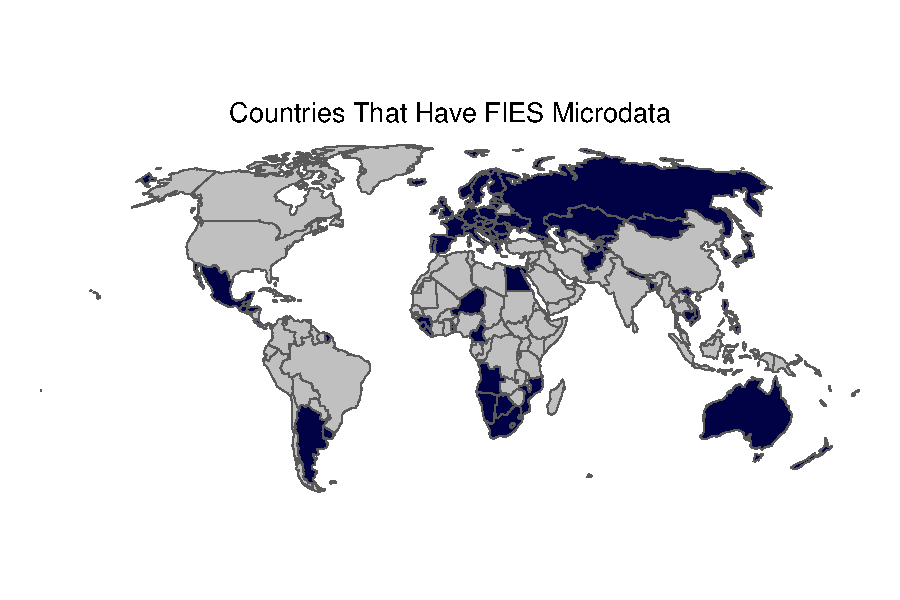
\includegraphics[width=\linewidth]{img/FIES_Countries.pdf}
  \caption{Countries used in our model, shown in blue.}
  \label{fig:fies_countries}
\end{figure}

The microdata includes information about the probability that an individual is over the threshold for moderate and severe food insecurity, calculated by the FAO on the basis of the responses to the 8 FIES questions (See List \ref{itm:fies}).  The FIES is calculated using a Rasch model, which was developed by the psychometrics literature.  The Rasch model assumes that each individual and their responses to the FIES questions can be placed on a one-dimensional scale of food insecurity, and that the log odds of a respondent answering affirmatively to one of the FIES questions is a linear function of the difference between the severity of the food insecurity experienced by the individual and the severity of the item put forward in the corresponding question.

The severity of each item and the respondent’s level of food insecurity can be estimated making use of maximum likelihood methods. The assumptions of the Rasch model hold up well for the data at hand, as evidenced by model fit diagnostics \cite{Cafiero2018}.

After separately estimating the Rasch model for each country, FAO develops a global reference scale for the severity of each of the eight questions by iteratively harmonizing the severity values in each country. These global reference points are calibrated against other surveys that ask questions similar to those in the FIES, such as the HFSSM and the ELCSA.

Based on the global reference scale, two thresholds are set based on questions 1 and 8, corresponding to moderate and severe food insecurity, respectively.


\begin{enumerate}
	\item During the last 12 months, was there a time when you were worried you would not have enough food to eat because of a lack of money or other resources?
	\item Still thinking about the last 12 months, was there a time when you were unable to eat healthy and nutritious food because of a lack of money or other resources?
	\item Was there a time when you ate only a few kinds of foods because of a lack of money or other resources?
	\item Was there a time when you had to skip a meal because there was not enough money or other resources to get food?
	\item Still thinking about the last 12 months, was there a time when you ate less than you thought you should because of a lack of money or other resources?
	\item Was there a time when your household ran out of food because of a lack of money or other resources?
	\item Was there a time when you were hungry but did not eat because there was not enough money or other resources for food?
	\item During the last 12 months, was there a time when you went without eating for a whole day because of a lack of money or other resources?
  \label{itm:fies}
\end{enumerate}

\section{Predicting Covariates Into the Future}
\subsection{Annualized Rate of Change}
For many of our covariates, to extrapolate recent trends to the future, we draw on historically annualized rates of change, which are used to project the future change in the variable. We use this method to estimate future rates of stunting, wasting, and malaria mortality, as well as to model future subnational shares of GDP and population.

For each subnational area, $a$, the rate of change (ROC) is calculated between each pair of adjacent years, $y$, based on a value, $p$, such that $0 < p < 1$, available for each year.

\begin{equation}
  \text{ROC}_{a,y} = \text{logit} \left( \frac{p_{a,y}}{p_{a,y-1}} \right)
  \label{eqn:a}
\end{equation}

Each ROC is weighted so as to give proportionally more weight to recent years.  For a dataset with observations for 2010 to 2019, that would be:

\begin{equation}
  W_y = \frac{y - 2010}{\sum_{y=2010}^{2019} y - 2010}
  \label{eqn:b}
\end{equation}

The annualized rate of change (AROC) is calculated as:

\begin{equation}
  \text{AROC}_{a} = \text{logit} \left( \sum_{y=2010}^{2019} W_y \times \text{AROC}_{a, y} \right)
  \label{eqn:c}
\end{equation}

Finally, the projections, Proj, for each year up to 2030 are given by:

\begin{equation}
  \text{Proj}_{a,y} = \text{logit}^{-1} ( \text{logit} ( p_{a,2019} ) + AROC_{a} \times ( y - 2019 ) )
  \label{eqn:d}
\end{equation}

For cases where we model shares with a summing constraint, such as the regional shares of a variable measured at the national level, we rescale the shares to ensure that the constraint holds.

\pagebreak
\subsection{Population}
Although population is not a covariate in our random forest model, it is an important determinant of other covariates such as GDP per capita. Future estimates of population are also necessary to convert modeled future rates of food insecurity into total headcounts of food insecurity. 

We project population by combining historical subnational data from the Subnational Development Database \citep{Smits2019} with national level population estimates for the 21st century \citep{KC2017}.  To account for within-country trends and changes in population distribution, we use the AROC method outlined in equations \ref{eqn:a} - \ref{eqn:d} to project each subnational areas share of national population totals. We then disaggregate the national totals given by KC et al. to estimate future subnational populations.

\begin{figure}[H]
  \centering
  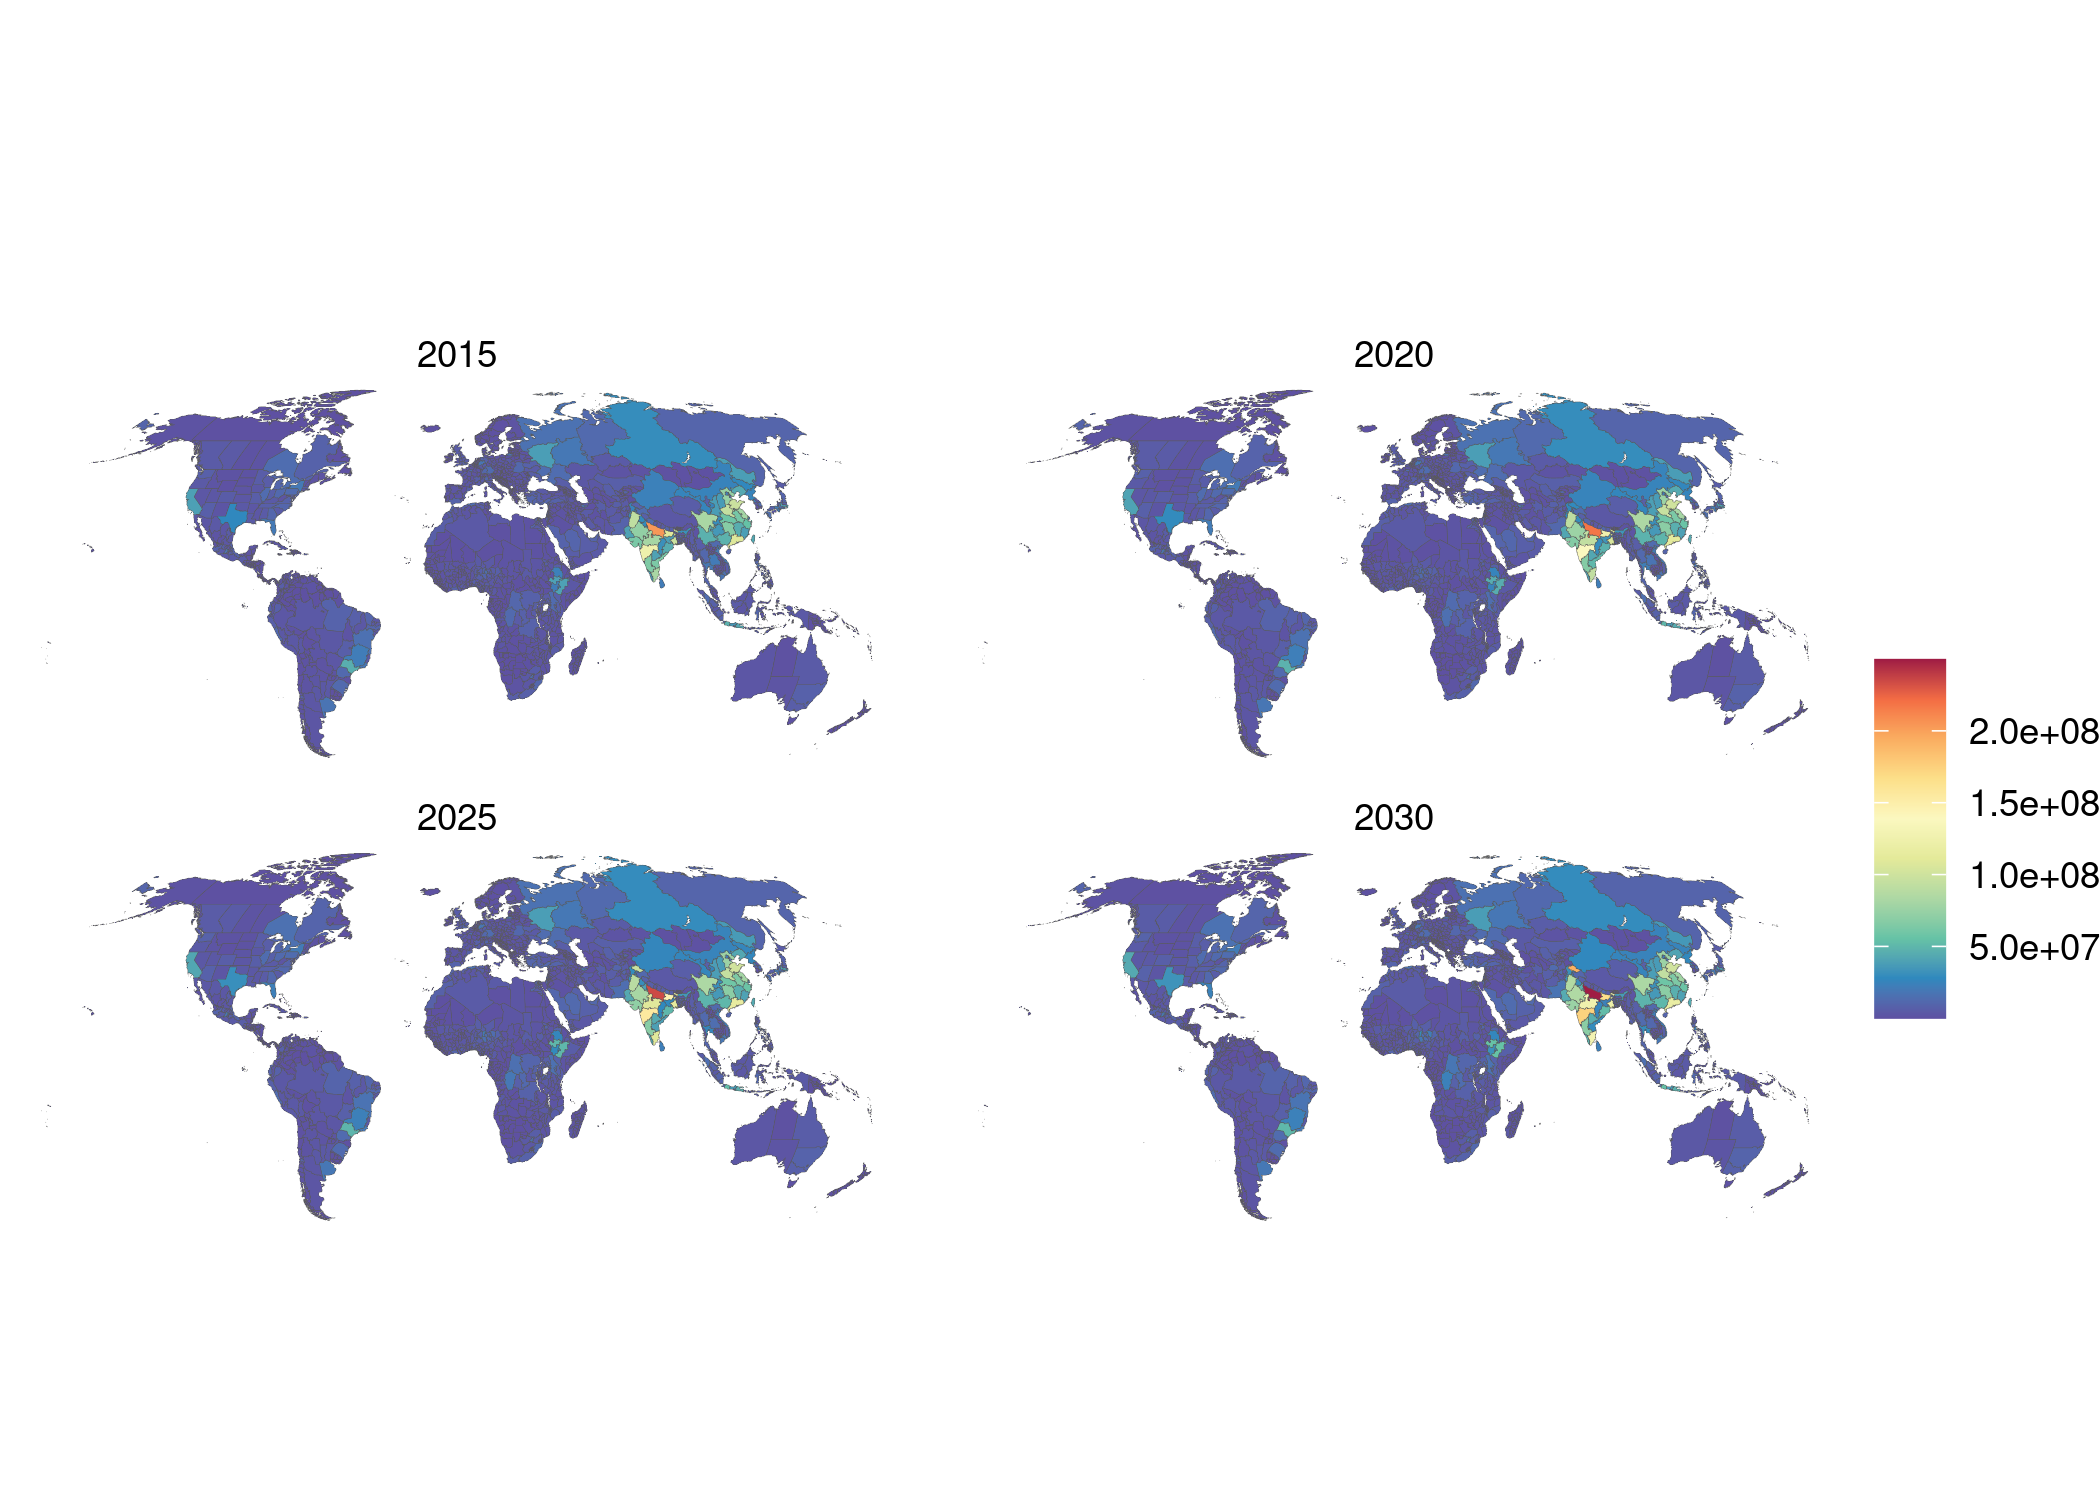
\includegraphics[width=\linewidth]{img/covars/population.png}
  \caption{Population}
\end{figure}

\pagebreak
\subsection{Urbanization Rates}

We draw our historical and future estimates of urbanization entirely from the spatially explicit scenarios of urban population by Jones and O'Neill \citep{Jones2016}, which provide a series of urbanization rate projections which are consistent with the Shared Socioeconomic Pathways.  As with our other covariates, we use projections consistent with SSP2, the middle-of-the-road scenario. 

\begin{figure}[H]
  \centering
  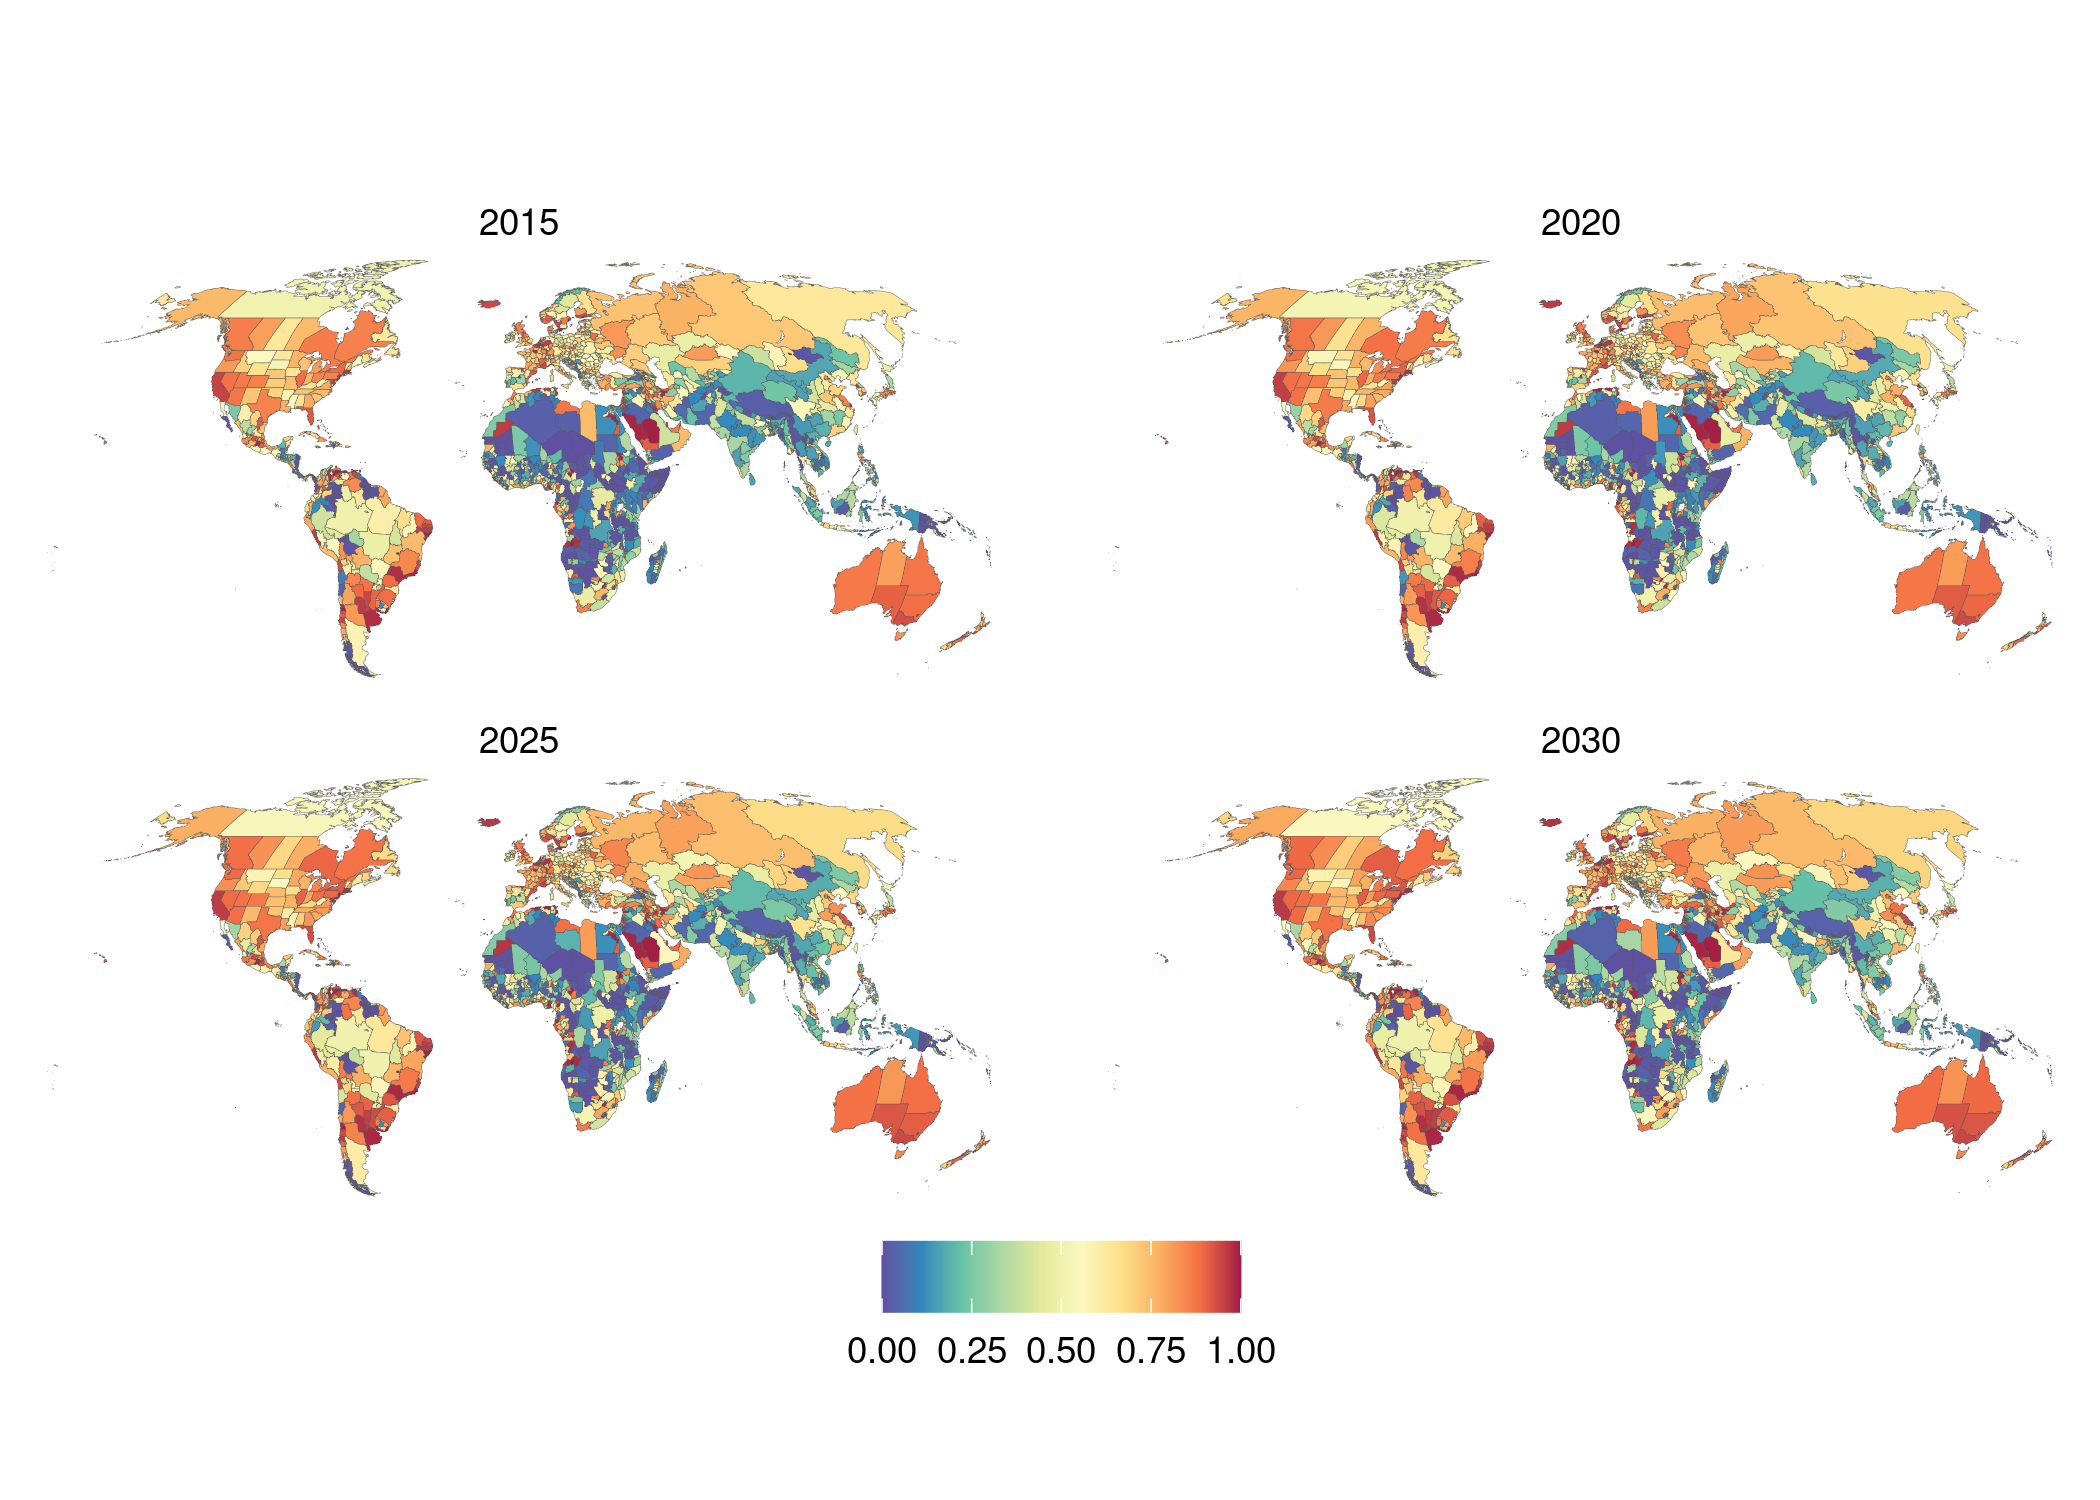
\includegraphics[width=\linewidth]{img/covars/urban_perc.png}
  \caption{Percentage of people living in urban areas.}
\end{figure}

\pagebreak
\subsection{Wasting}
To estimate the prevalence of wasting for each administrative area in our dataset, we use data from the Local Burden of Disease project.  For the years 2010 to 2017, we simply use the mean rate of wasting in each administrative area from the dataset.  Higher-income countries that are not included in the dataset are assumed to have zero wasting.  We then project wasting for the years 2018-2030 using the AROC method, which the Local Burden of Disease group similarly use to estimate wasting for the year 2025 \citep{Local2020}.

To account for the effects of the coronavirus pandemic on global rates of wasting, we assume that long-term trends in rates of wasting would hold steady, after they increase globally by 14.3\% in 2020, based on estimates published in \textit{The Lancet} \citep{headey2020impacts}.  We model this impact as uniform across all countries where wasting occurs.  We project the rate of wasting in each administrative area in 2021 as being the average of (a) the rate of change in 2020 accounting for the pandemic shock and (b) the predicted rate of change for 2022 obtained ignoring the pandemic.

\begin{figure}[H]
  \centering
  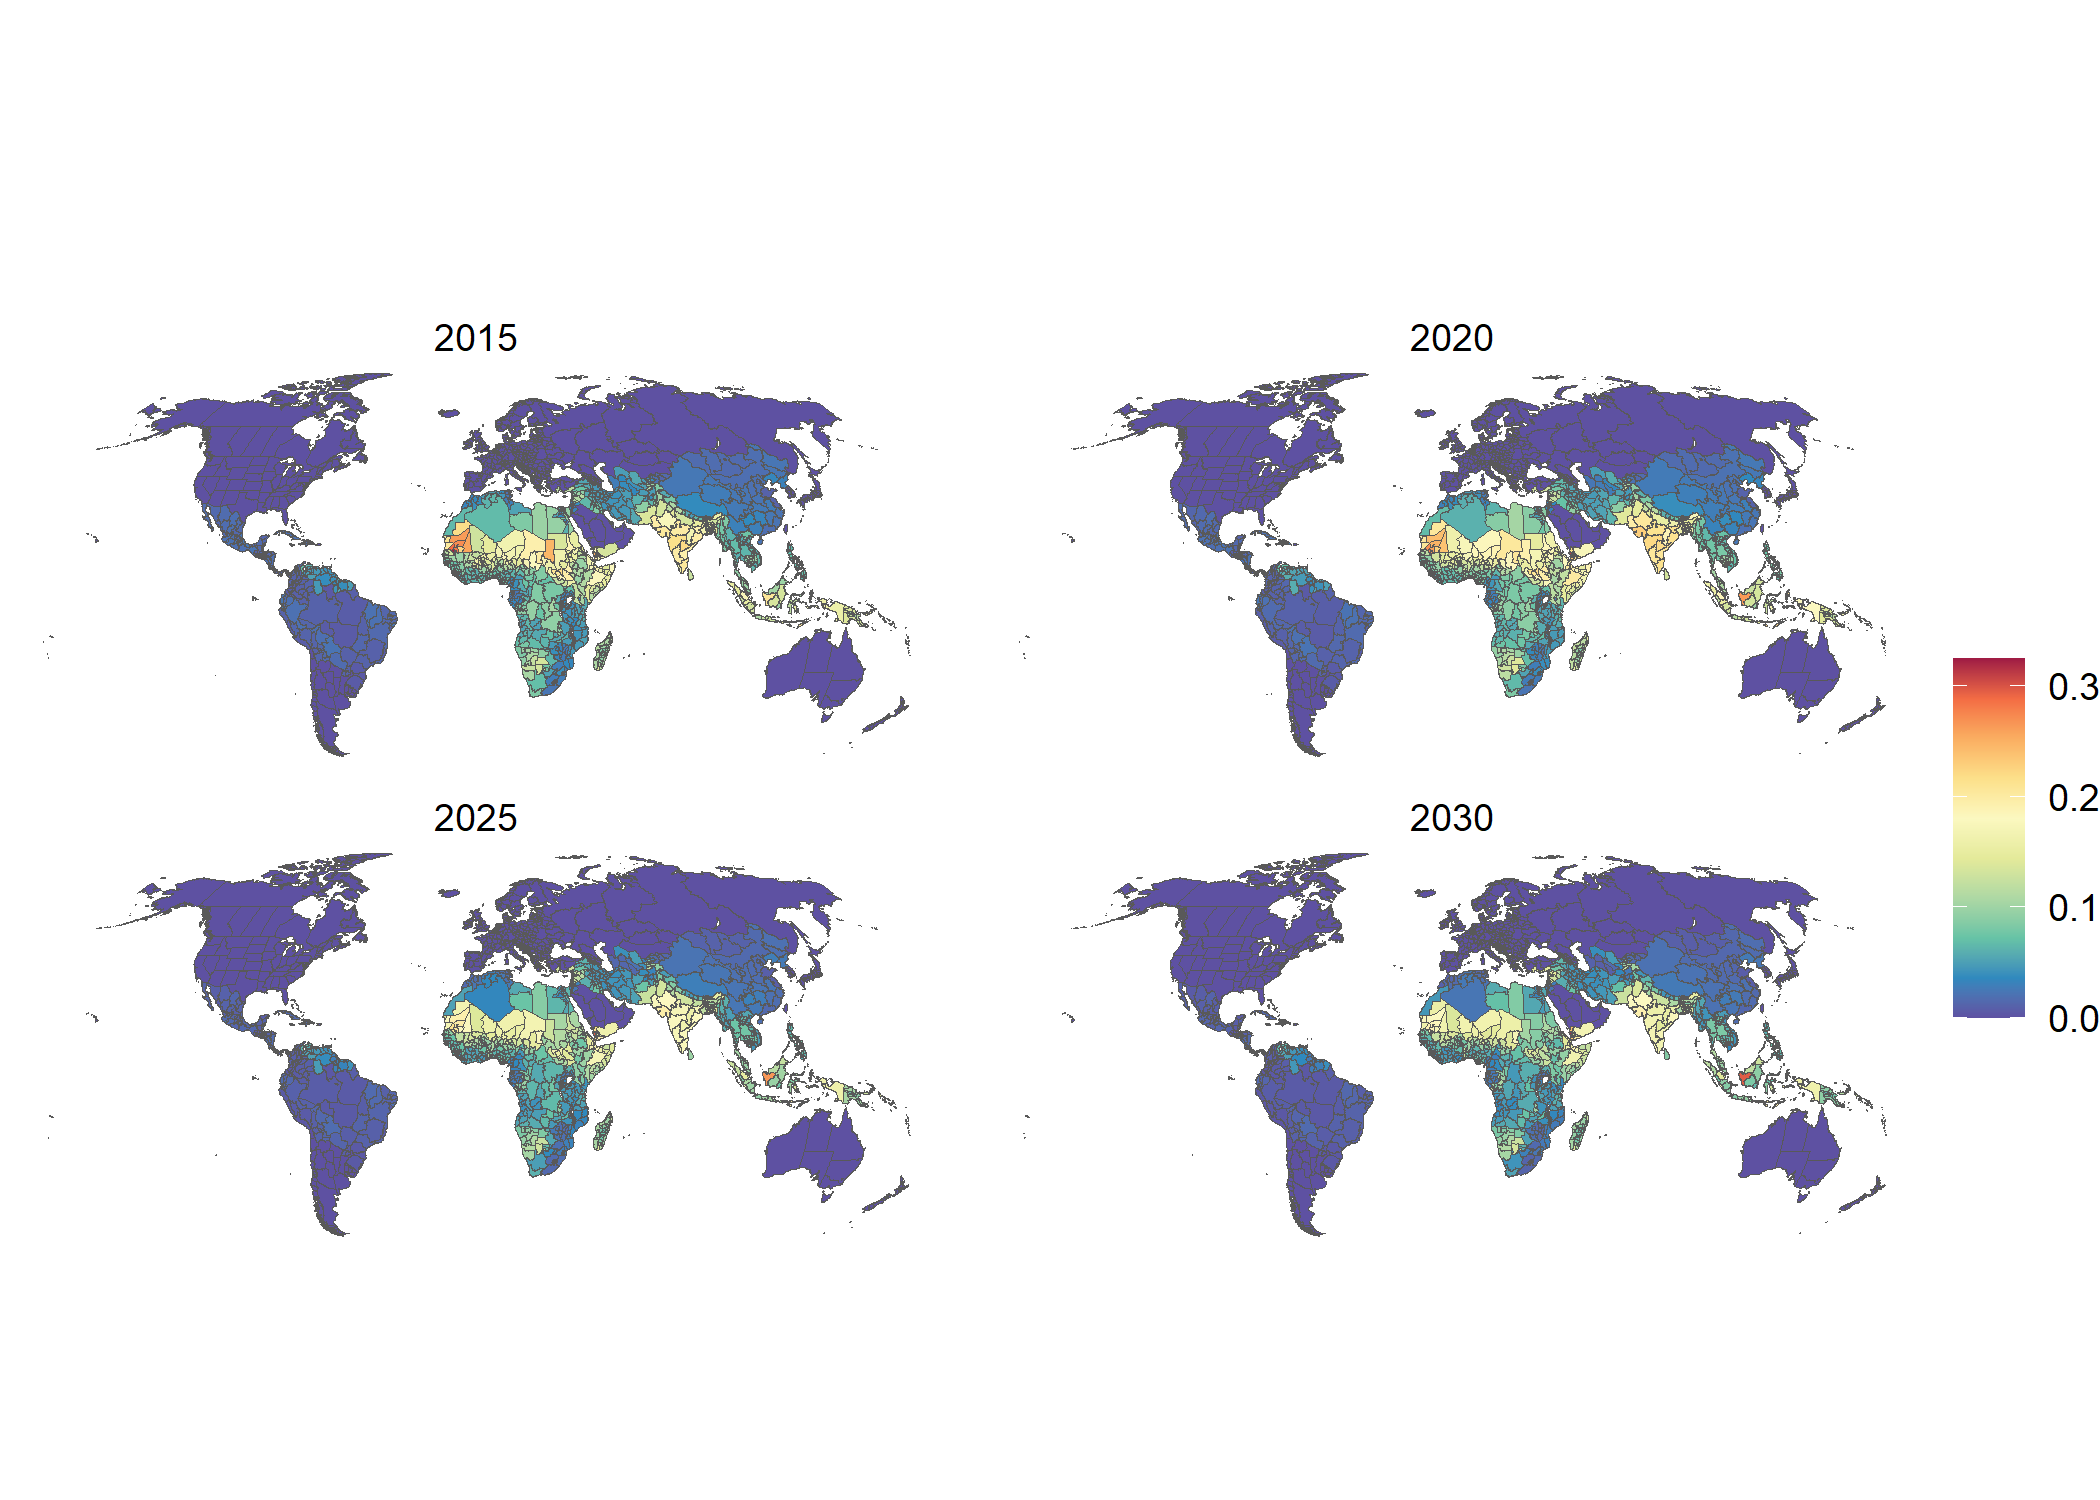
\includegraphics[width=\linewidth]{img/covars/wasting.png}
  \caption{Prevalence of wasting.}
\end{figure}

\pagebreak
\subsection{Stunting}
We model stunting, sourced from the Local Burden of Disease dataset, using the same methodology employed for wasting. We also assume a 14.3\% increase in prevalence for the year 2020 \citep{headey2020impacts}, as is done for wasting, although stunting is a long-term consequence of malnutrition and is not likely to be observable in a population with the same lags as wasting would be. We use stunting in our modeling framework as a proxy for chronic conditions of hunger, which are probably exacerbated by the coronavirus pandemic. 

\begin{figure}[H]
  \centering
  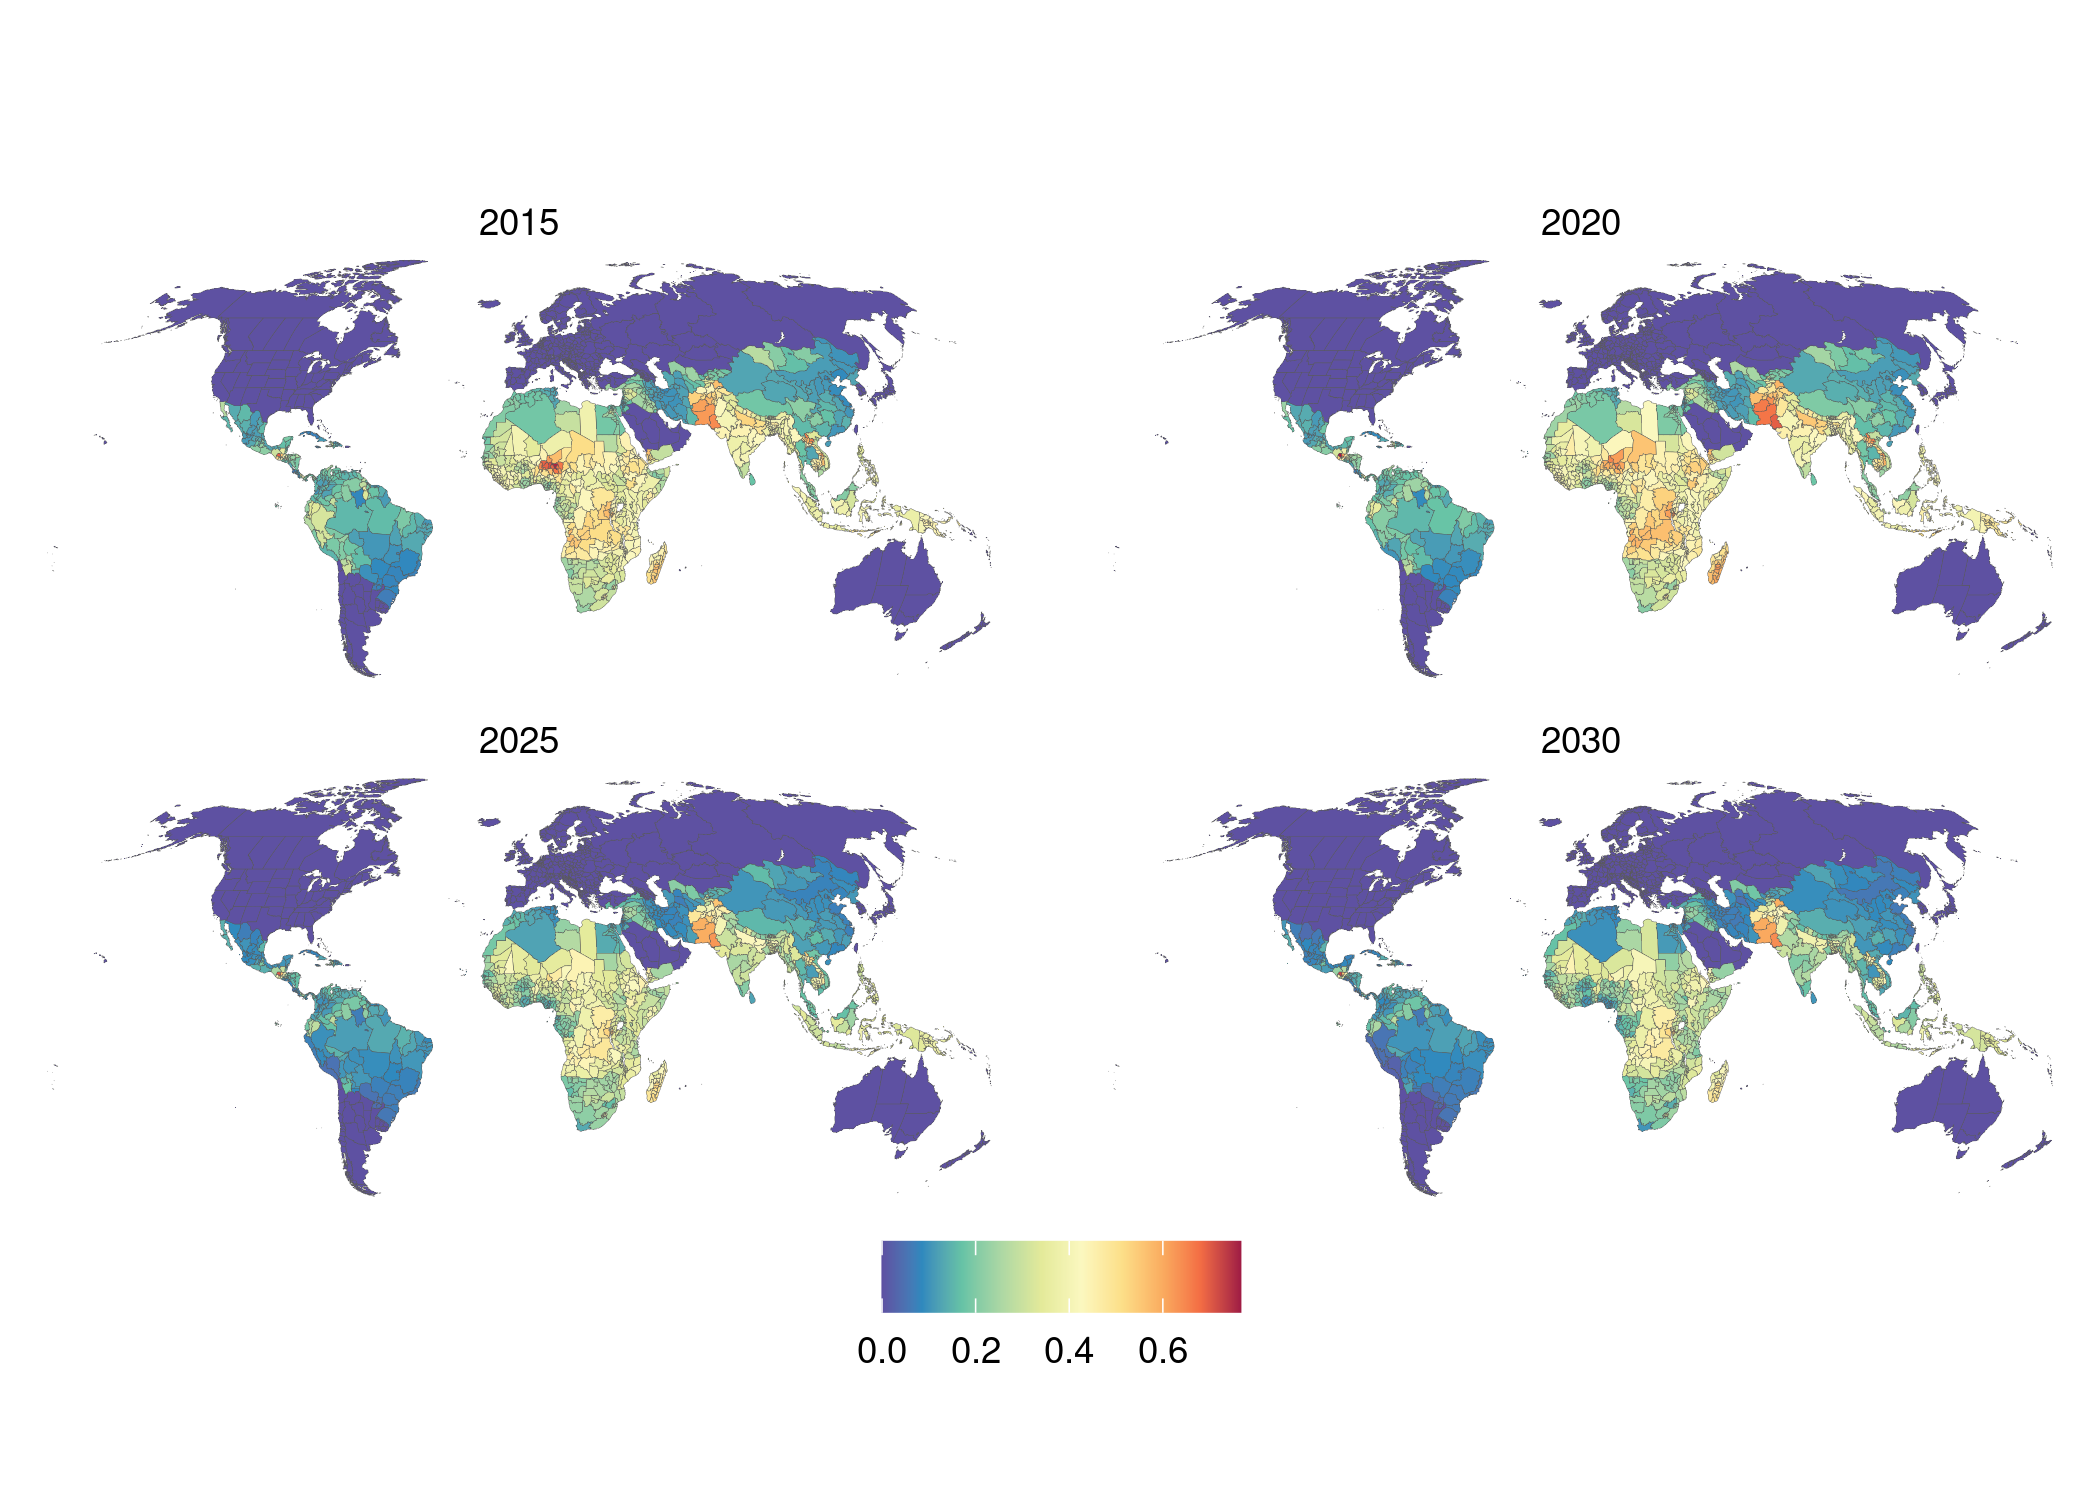
\includegraphics[width=\linewidth]{img/covars/stunting.png}
  \caption{Prevalence of stunting.}
\end{figure}

\pagebreak
\subsection{GDP Per Capita}
We estimate global subnational GDP per capita using historic subnational estimates of Gross National Income (GNI) from the Subnational Human Development Database \cite{Smits2019} and forecasts of national GDP within the SSP framework from Dellink et al. \cite{Dellink2017}.  We first use data from the World Bank to estimate the mean country-level ratio of GNI to GDP and adjust the subnational estimates of GNI according to that country-specific ratio.  We then calculate each subnational area's share of country GDP, and then use the AROC method to estimate each subnational area's share of total country GDP.  Based on these trajectories in each subnational areas share of total country GDP, we estimate what each subnational area's share of GDP will be for each year from 2019 to 2030.  We divide that share of GDP by the population of the administrative area, which we had previously estimated.  Thus, national GDP totals are consistent with the projections of Dellink et al., but are disaggregated according to the historic patters of GDP share in the Subnational Human Development Database.

Finally, we used estimates of country-level changes in GDP growth for the years 2020 and 2021 to account for the impact of the coronavirus \citep{prospects2020}.  We then model GDP as resuming its previous growth trajectory based on previously-estimated growth rates from 2022-2030, but growing from an estimate for 2021 that includes the coronavirus shock.

We measure global subnational GDP per capita using historic subnational estimates of Gross National Income (GNI) from the Subnational Human Development Database \citep{Smits2019} and forecasts of national GDP within the SSP framework form Dellink et al. \citep{Dellink2017}. We source data on the mean country-level ratio of GNI to GDP from the World Bank and adjust the subnational estimates of GNI according to the ratio for each country in our sample. We calculate the share of national GDP for each subnational region, and use the AROC method to project each subnational area’s share of total country GDP up to 2030. National GDP totals are consistent with the projections of Dellink et al., but are disaggregated according to the historic patterns of subnational GDP shares sourced from the Subnational Human Development Database. We use nowcasts and forecasts of country-level changes in GDP growth for the years 2020 and 2021 to account for the impact of the coronavirus \citep{prospects2020}. After the shock created by the COVID pandemic, GDP is assumed to resuming its previous growth trajectory for the period 2022-2030.

\begin{figure}[H]
  \centering
  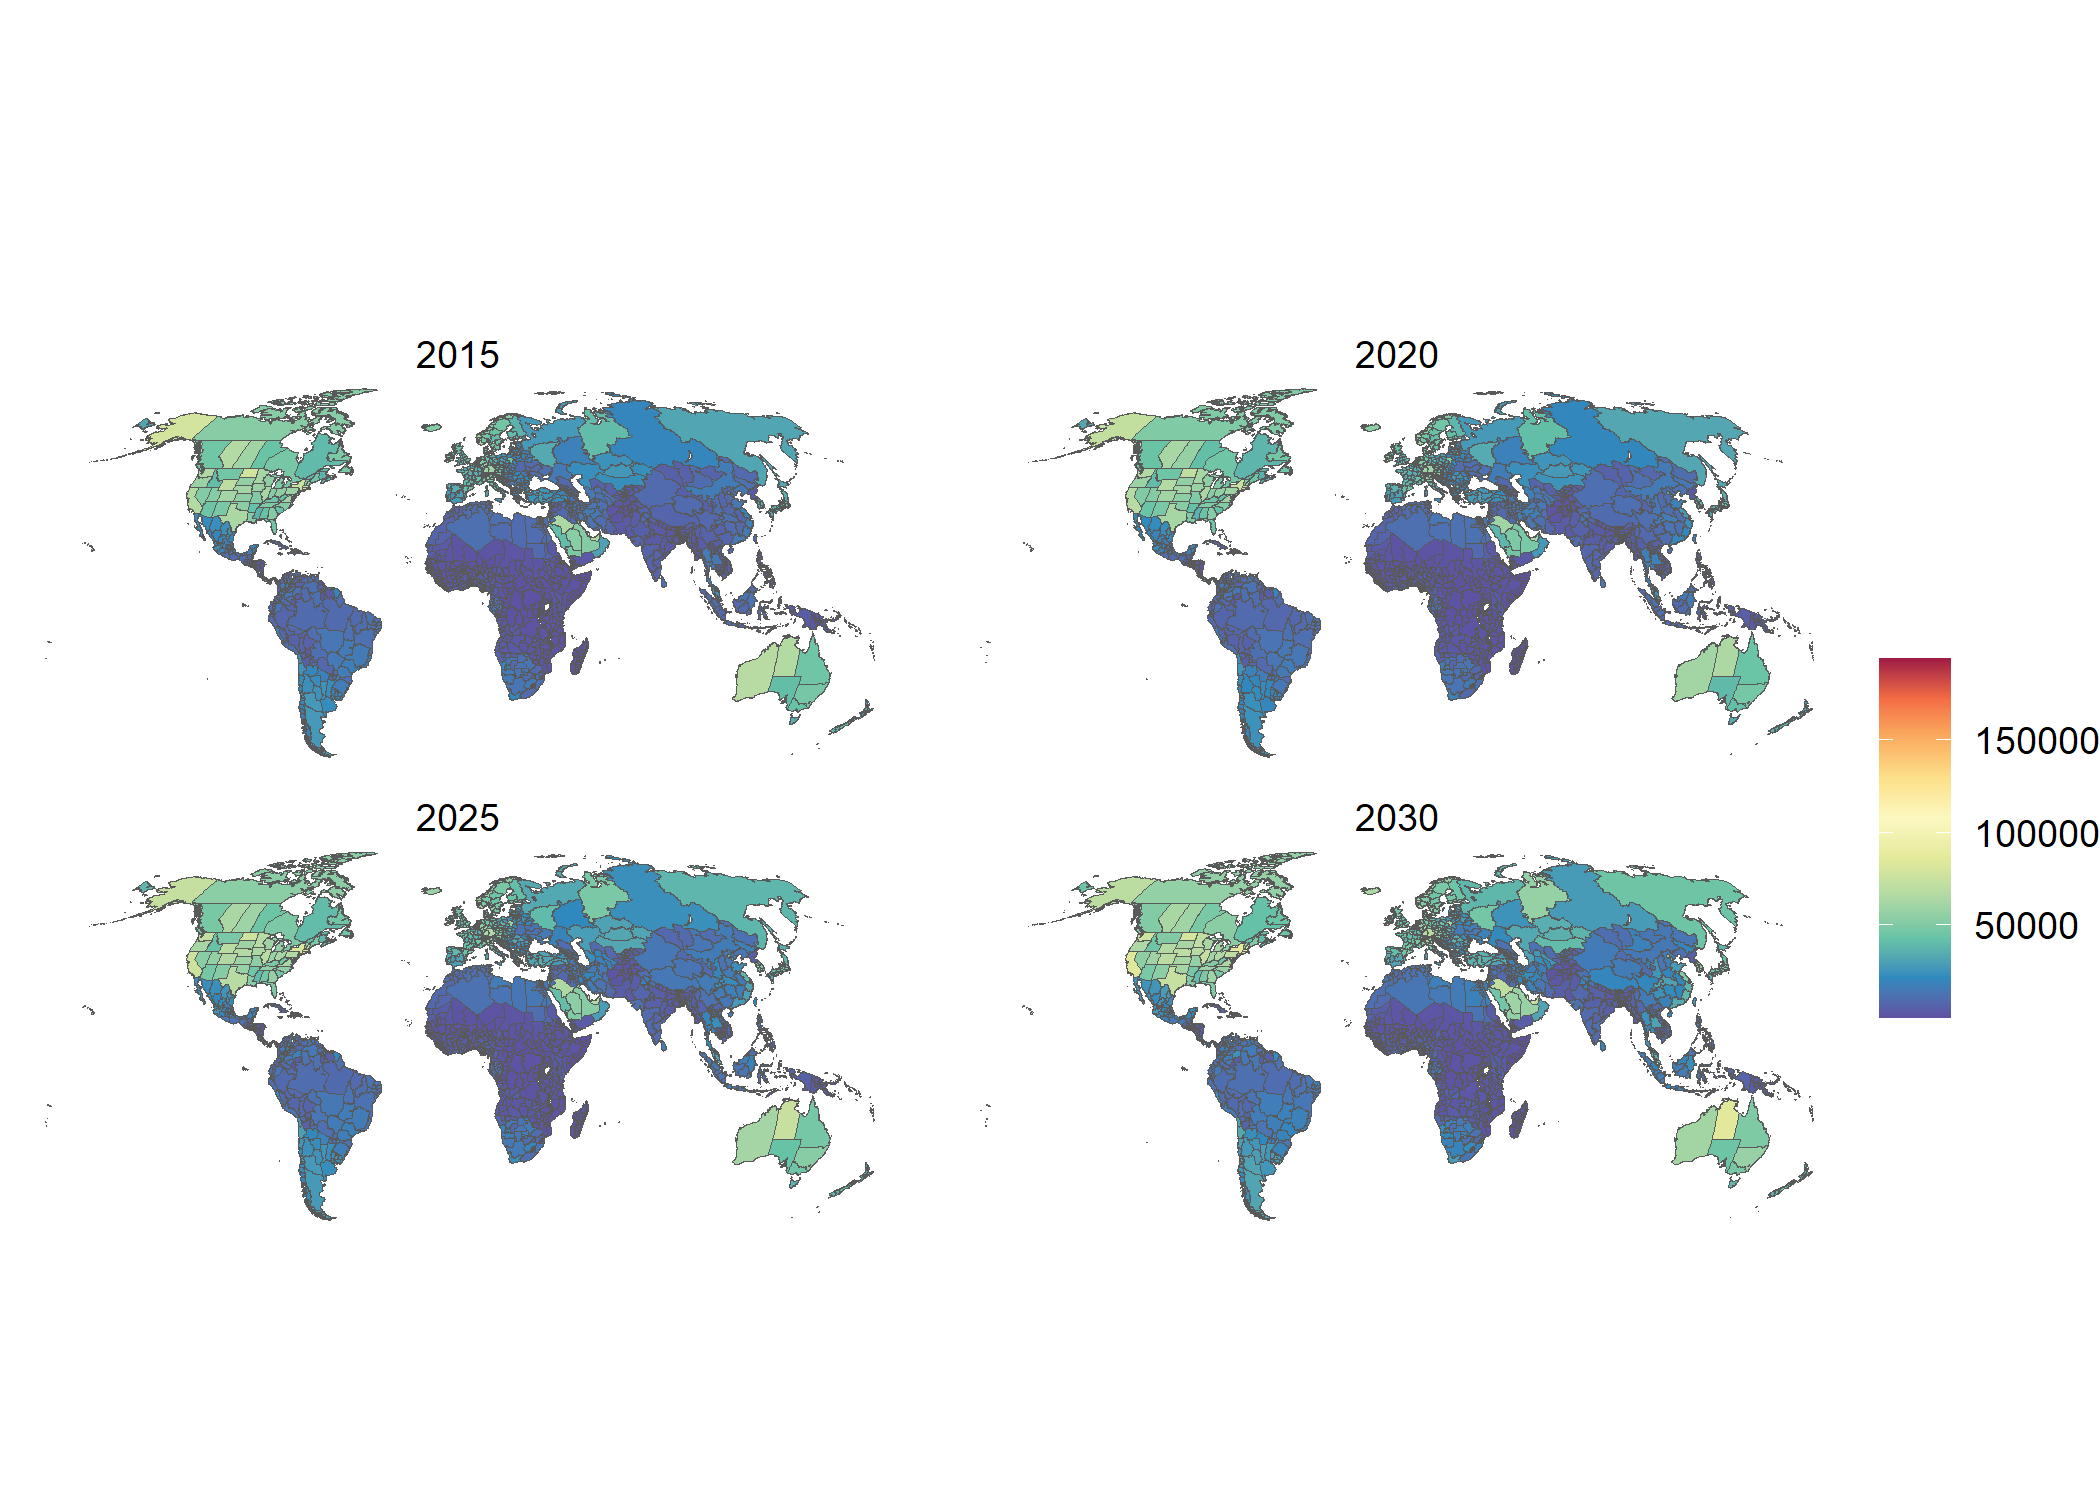
\includegraphics[width=\linewidth]{img/covars/gdp_percap.png}
  \caption{GDP per capita.}
\end{figure}

\pagebreak
\subsection{Mean Years of Schooling}
We use data on global subnational mean years of schooling from the Subnational Human Development Database \cite{Smits2019} and forecasts of national mean years of schooling from KC et al. \cite{KC2017}.  Using the subnational data, we calculate the difference in years of schooling form the nation mean each subnational administrative area, and use this value to disaggregate the future projections to a subnational level, keeping these differences constant over the projection horizon.


\begin{figure}[H]
  \centering
  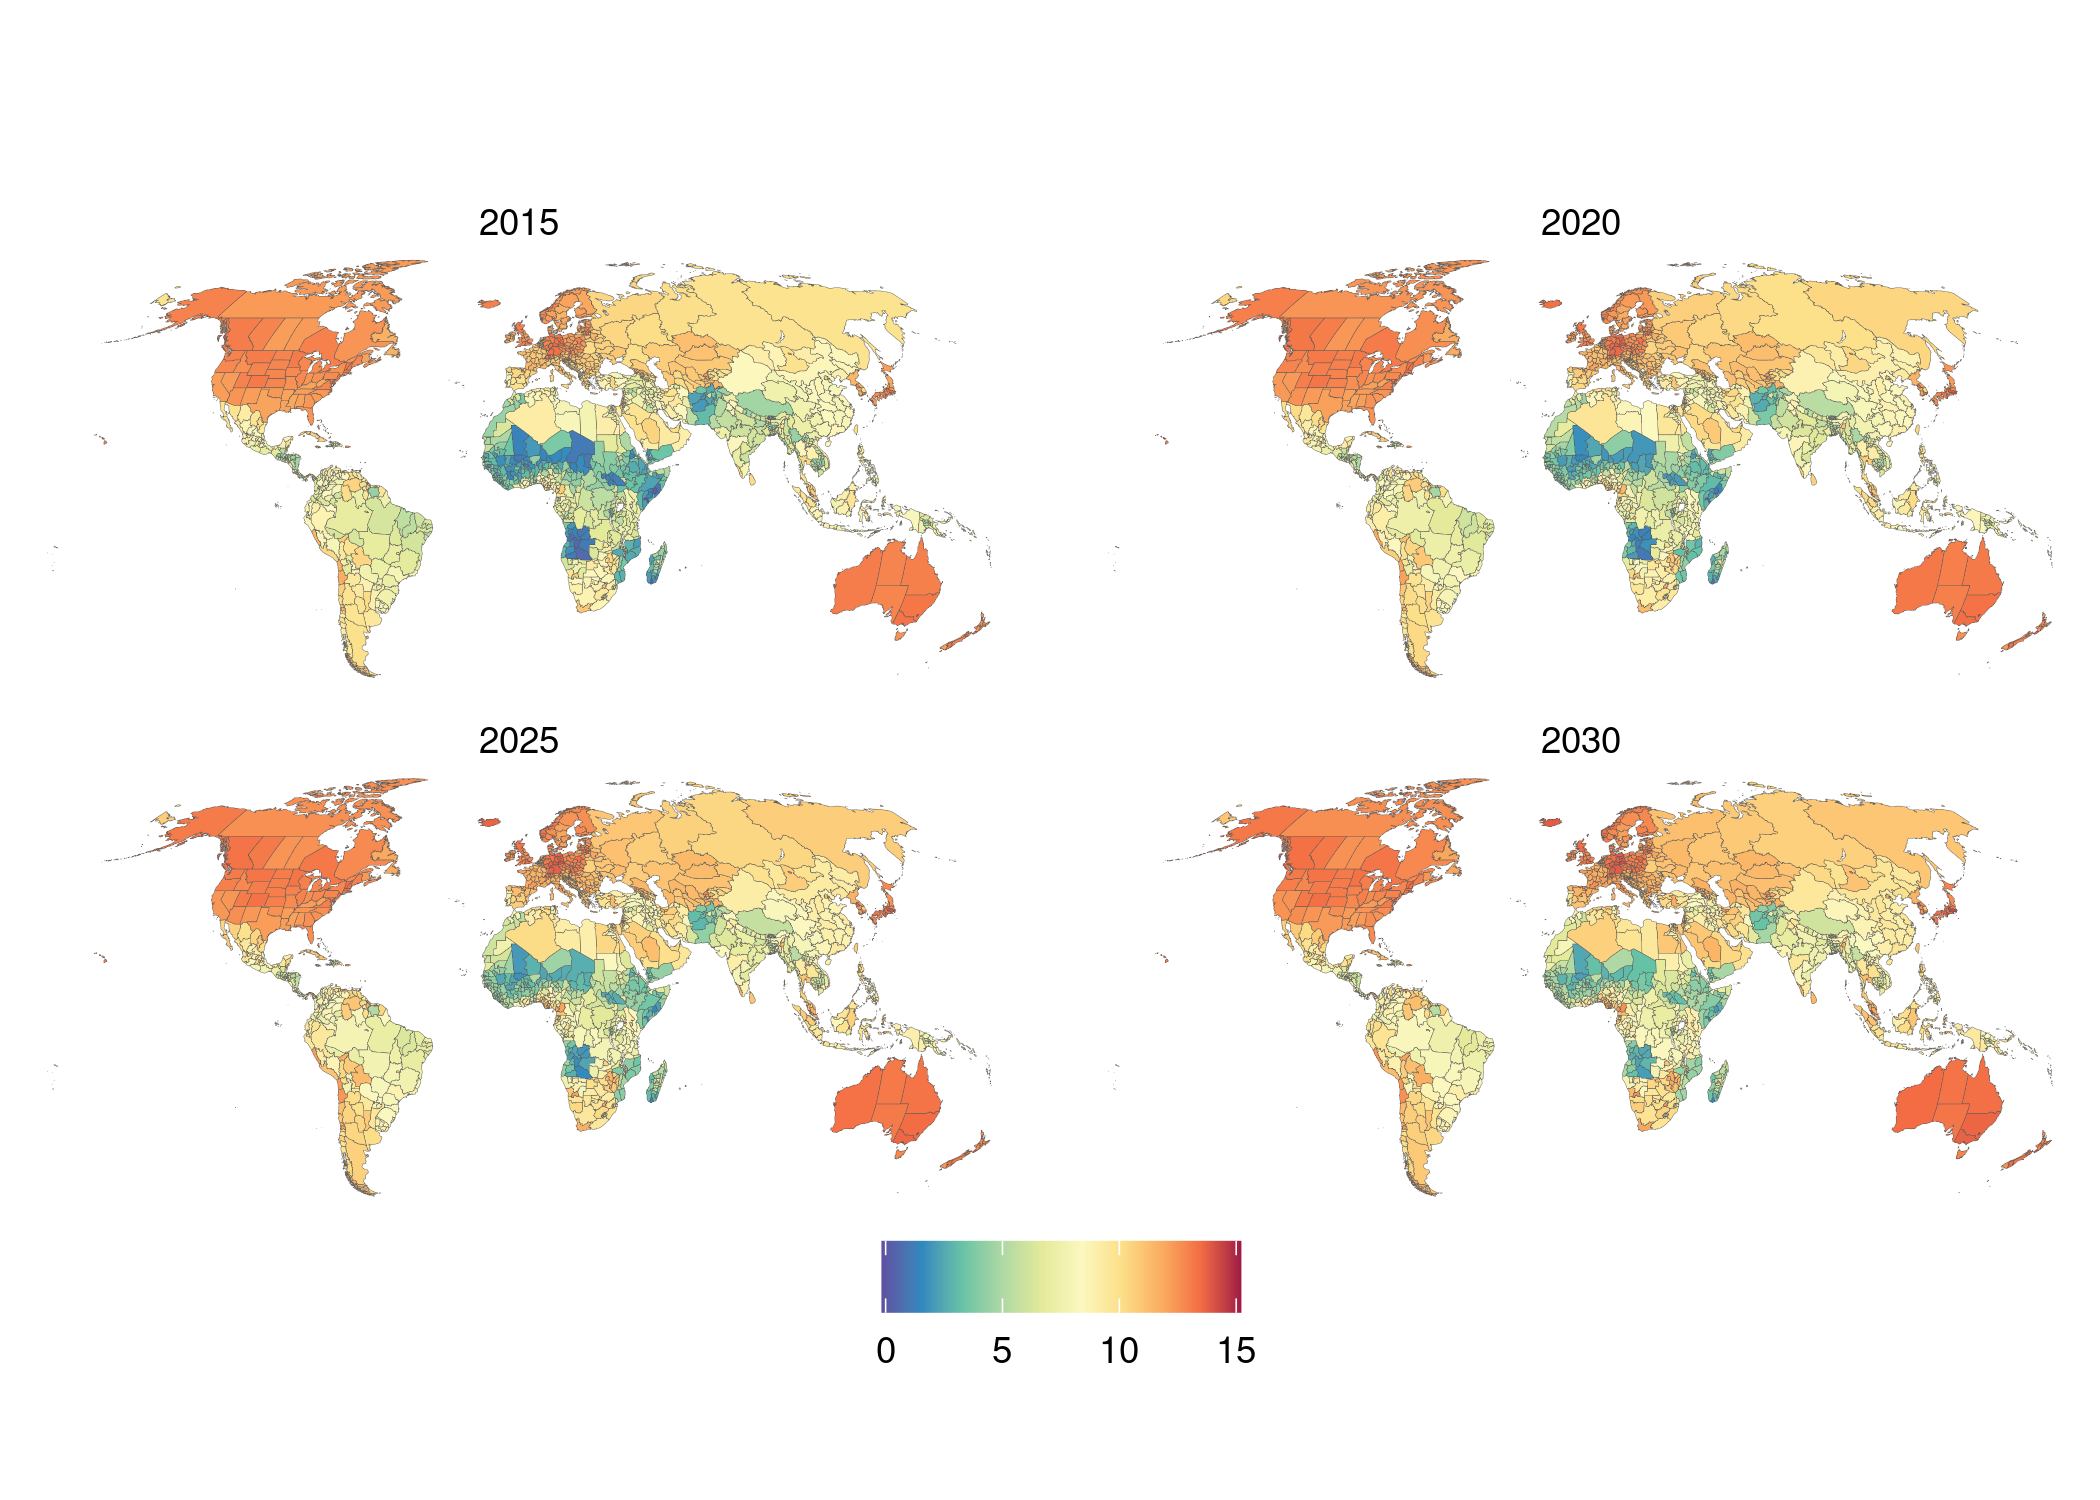
\includegraphics[width=\linewidth]{img/covars/school_mean.png}
  \caption{Mean years of schooling.}
\end{figure}


\pagebreak
\subsection{Gini Coefficient}
We use data on historical levels and projections of national income inequality from Rao et al. \citep{Rao2019a}.  These estimates are not disaggregated to a subnational level.

\begin{figure}[H]
  \centering
  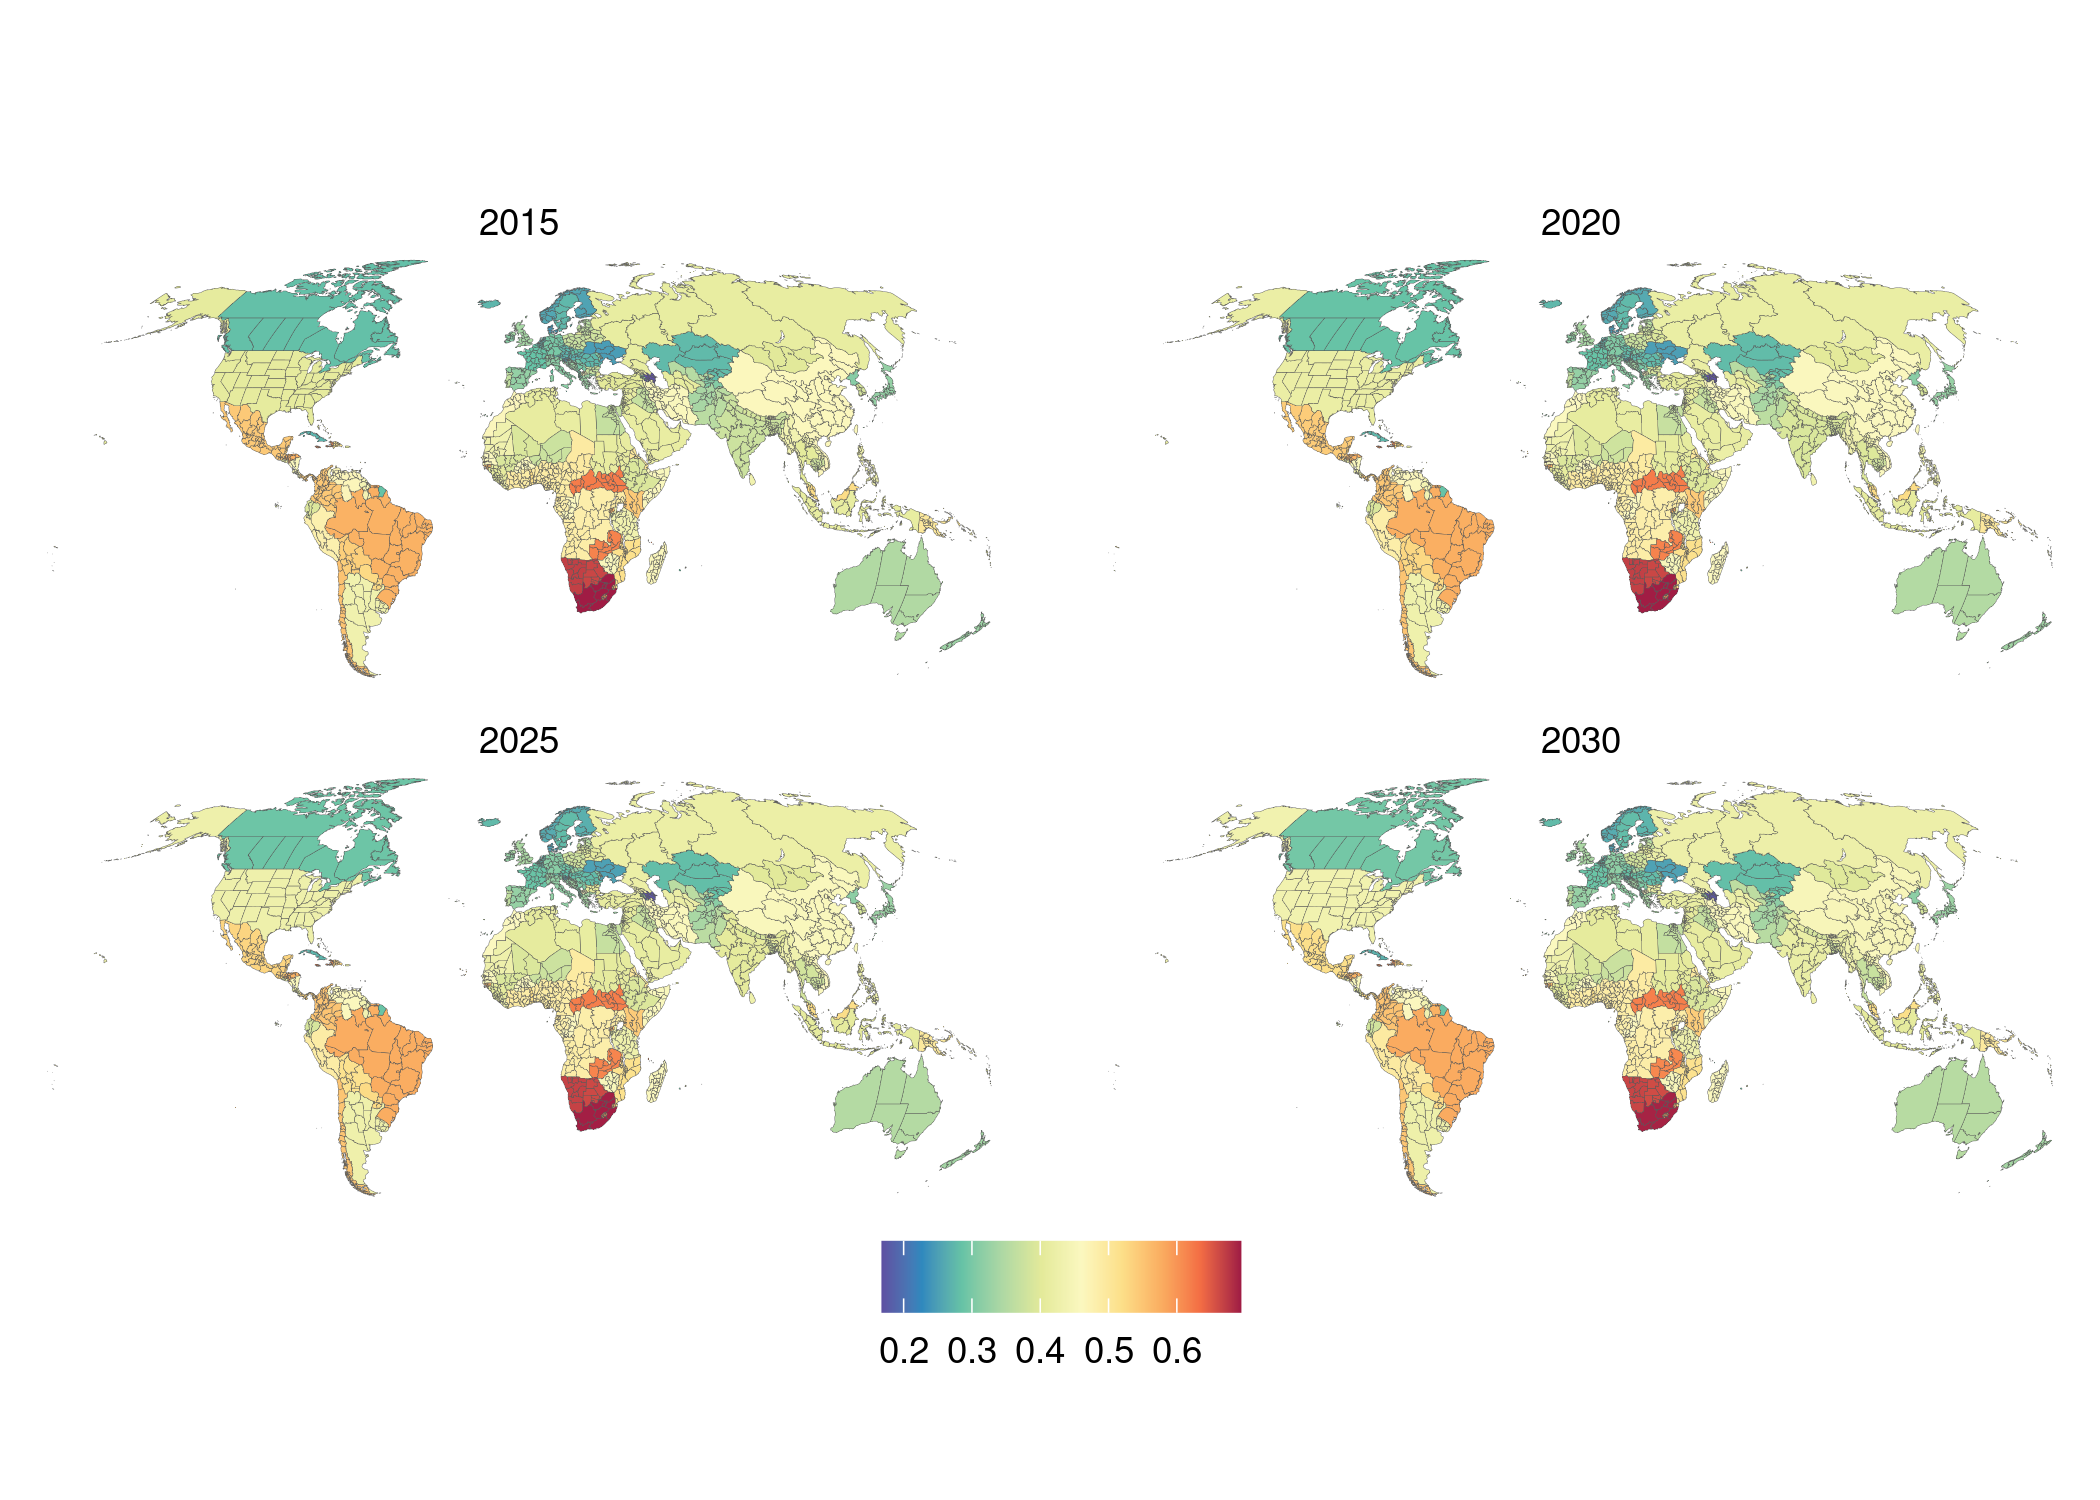
\includegraphics[width=\linewidth]{img/covars/gini.png}
  \caption{Gini Coefficient}
\end{figure}

\pagebreak
\subsection{Poverty Headcount Index}
We used historical and projected data on the Poverty Headcount Index (using the standard threshold of \$1.90 a day) from the World Poverty Clock by the World Data Lab, which in turn uses Povcal data sourced from the World Bank \citep{Cuaresma2018}. These data are the version corresponding to the update in summer 2020 and include the expected impact of the COVID pandemic on global poverty dynamics. Using parameterized Lorenz curves in combination with mean income/consumption and population projections, poverty rates are projected. 

\begin{figure}[H]
  \centering
  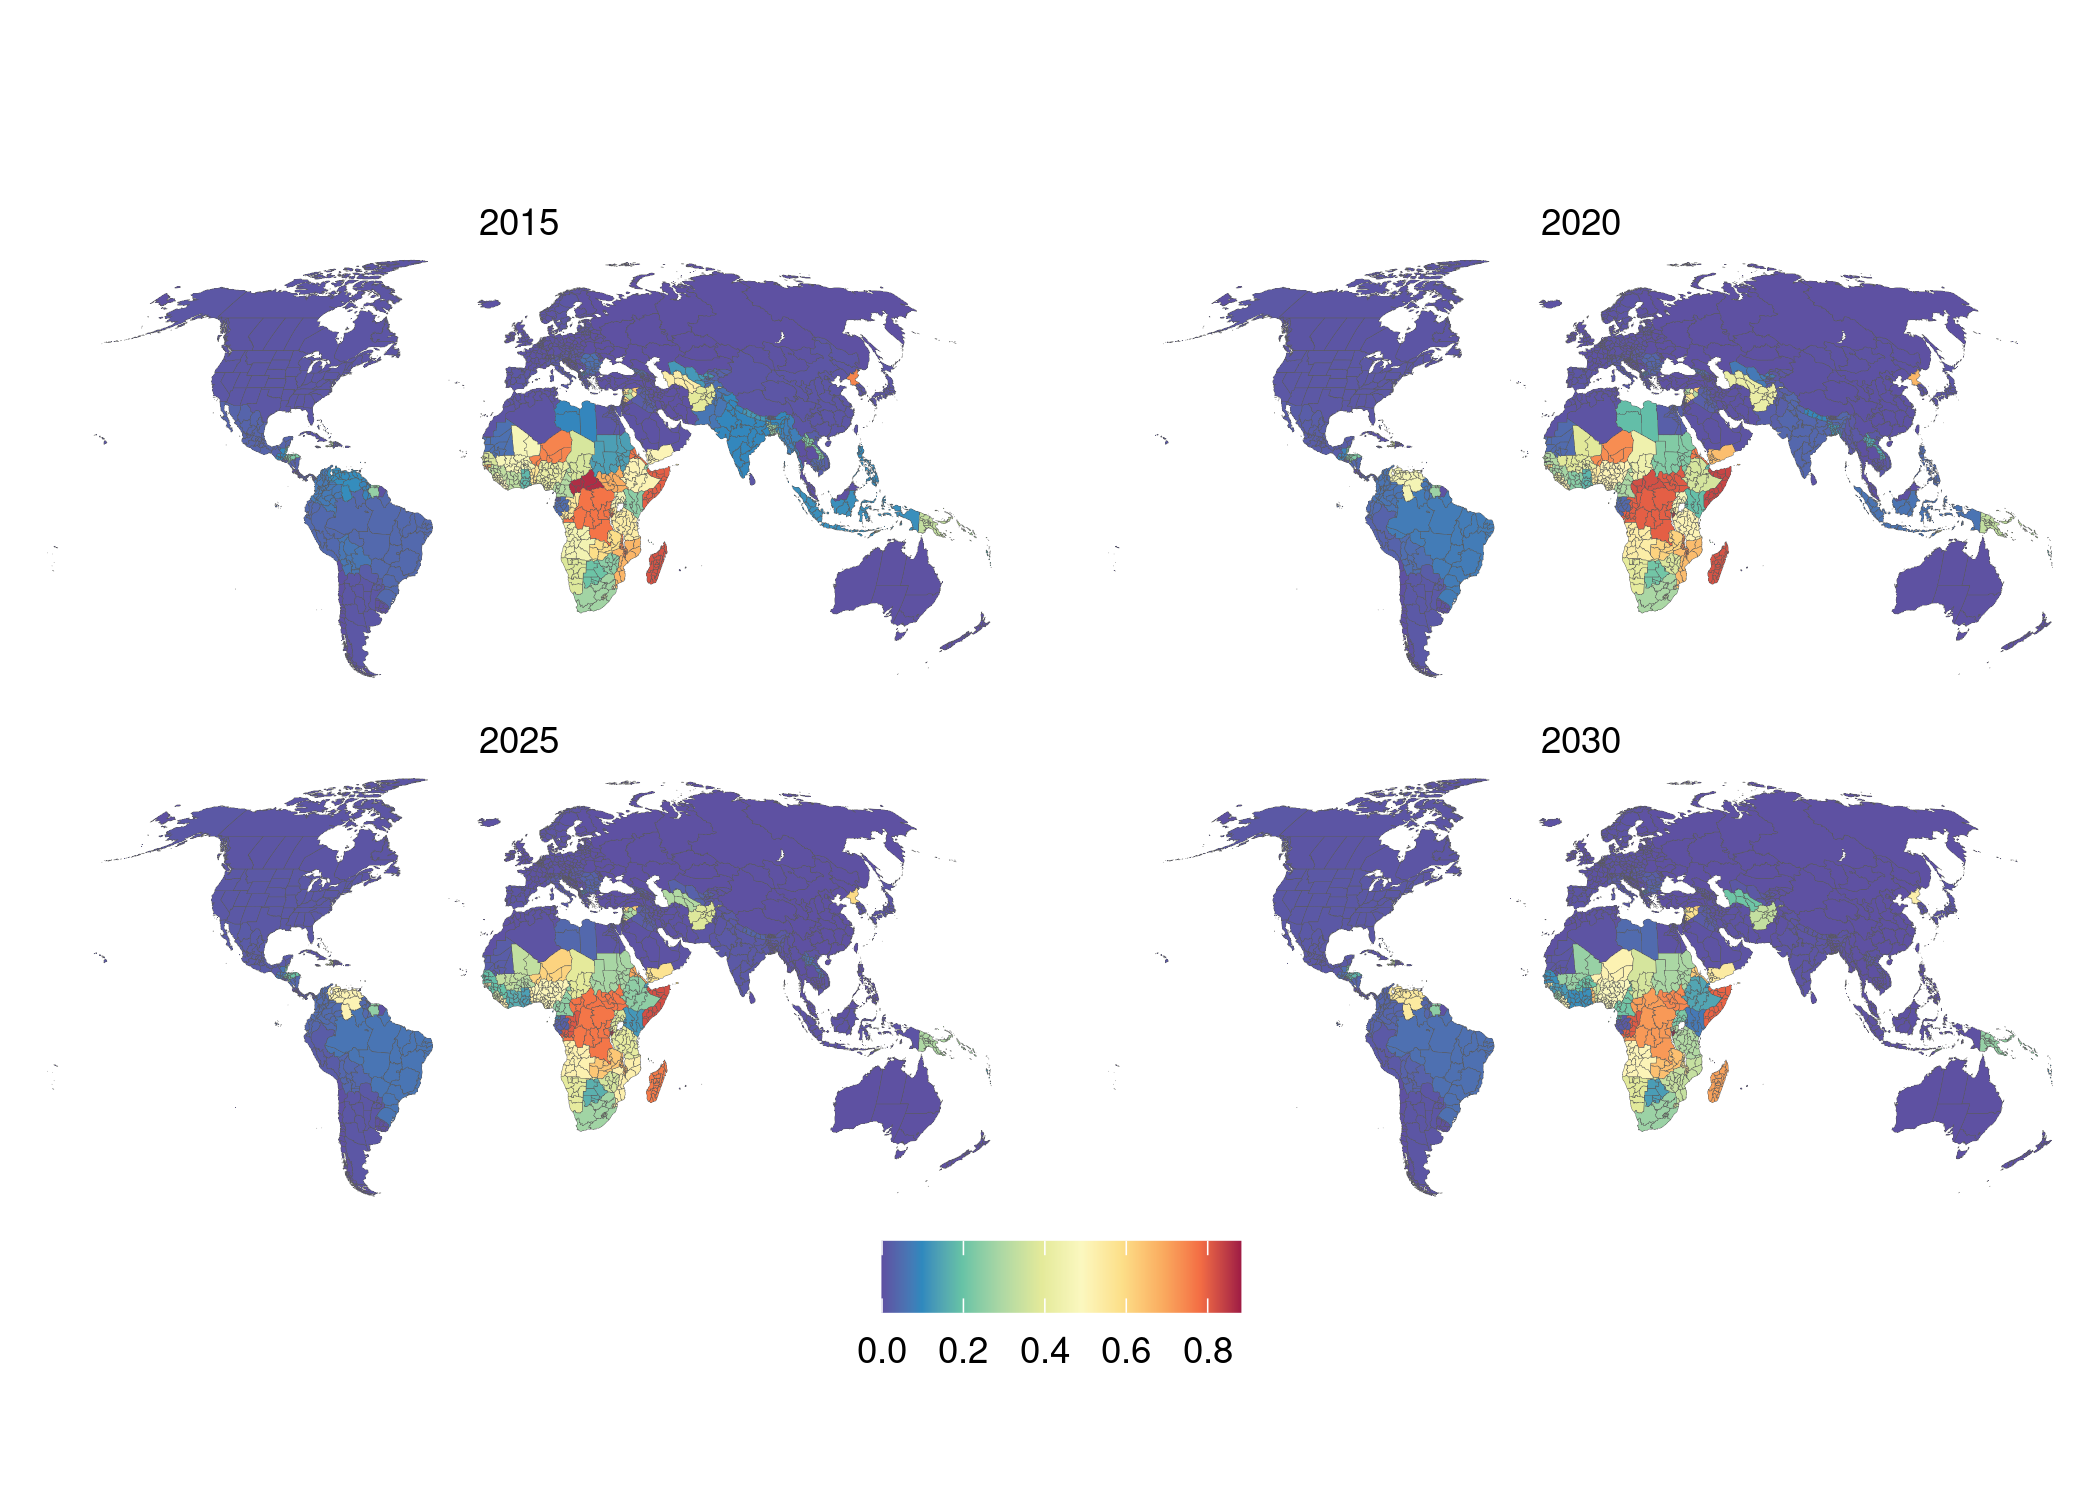
\includegraphics[width=\linewidth]{img/covars/hci.png}
  \caption{Poverty Headcount Index}
\end{figure}

\pagebreak
\subsection{Water Scarcity}
We use data for the water scarcity index (WSI) developed by \citep{greve2018global}. The index represents the ratio of the decadal averages in water demand to water supply, based on population projections consistent with SSP2 and water availability projections from global hydrological and general circulation models.  Based on this index, we estimate the share of people living in areas with less than 1000m\textsuperscript{3} of water available per capita per year. The WSI has been used already to build the water scarcity clock.

\begin{figure}[H]
  \centering
  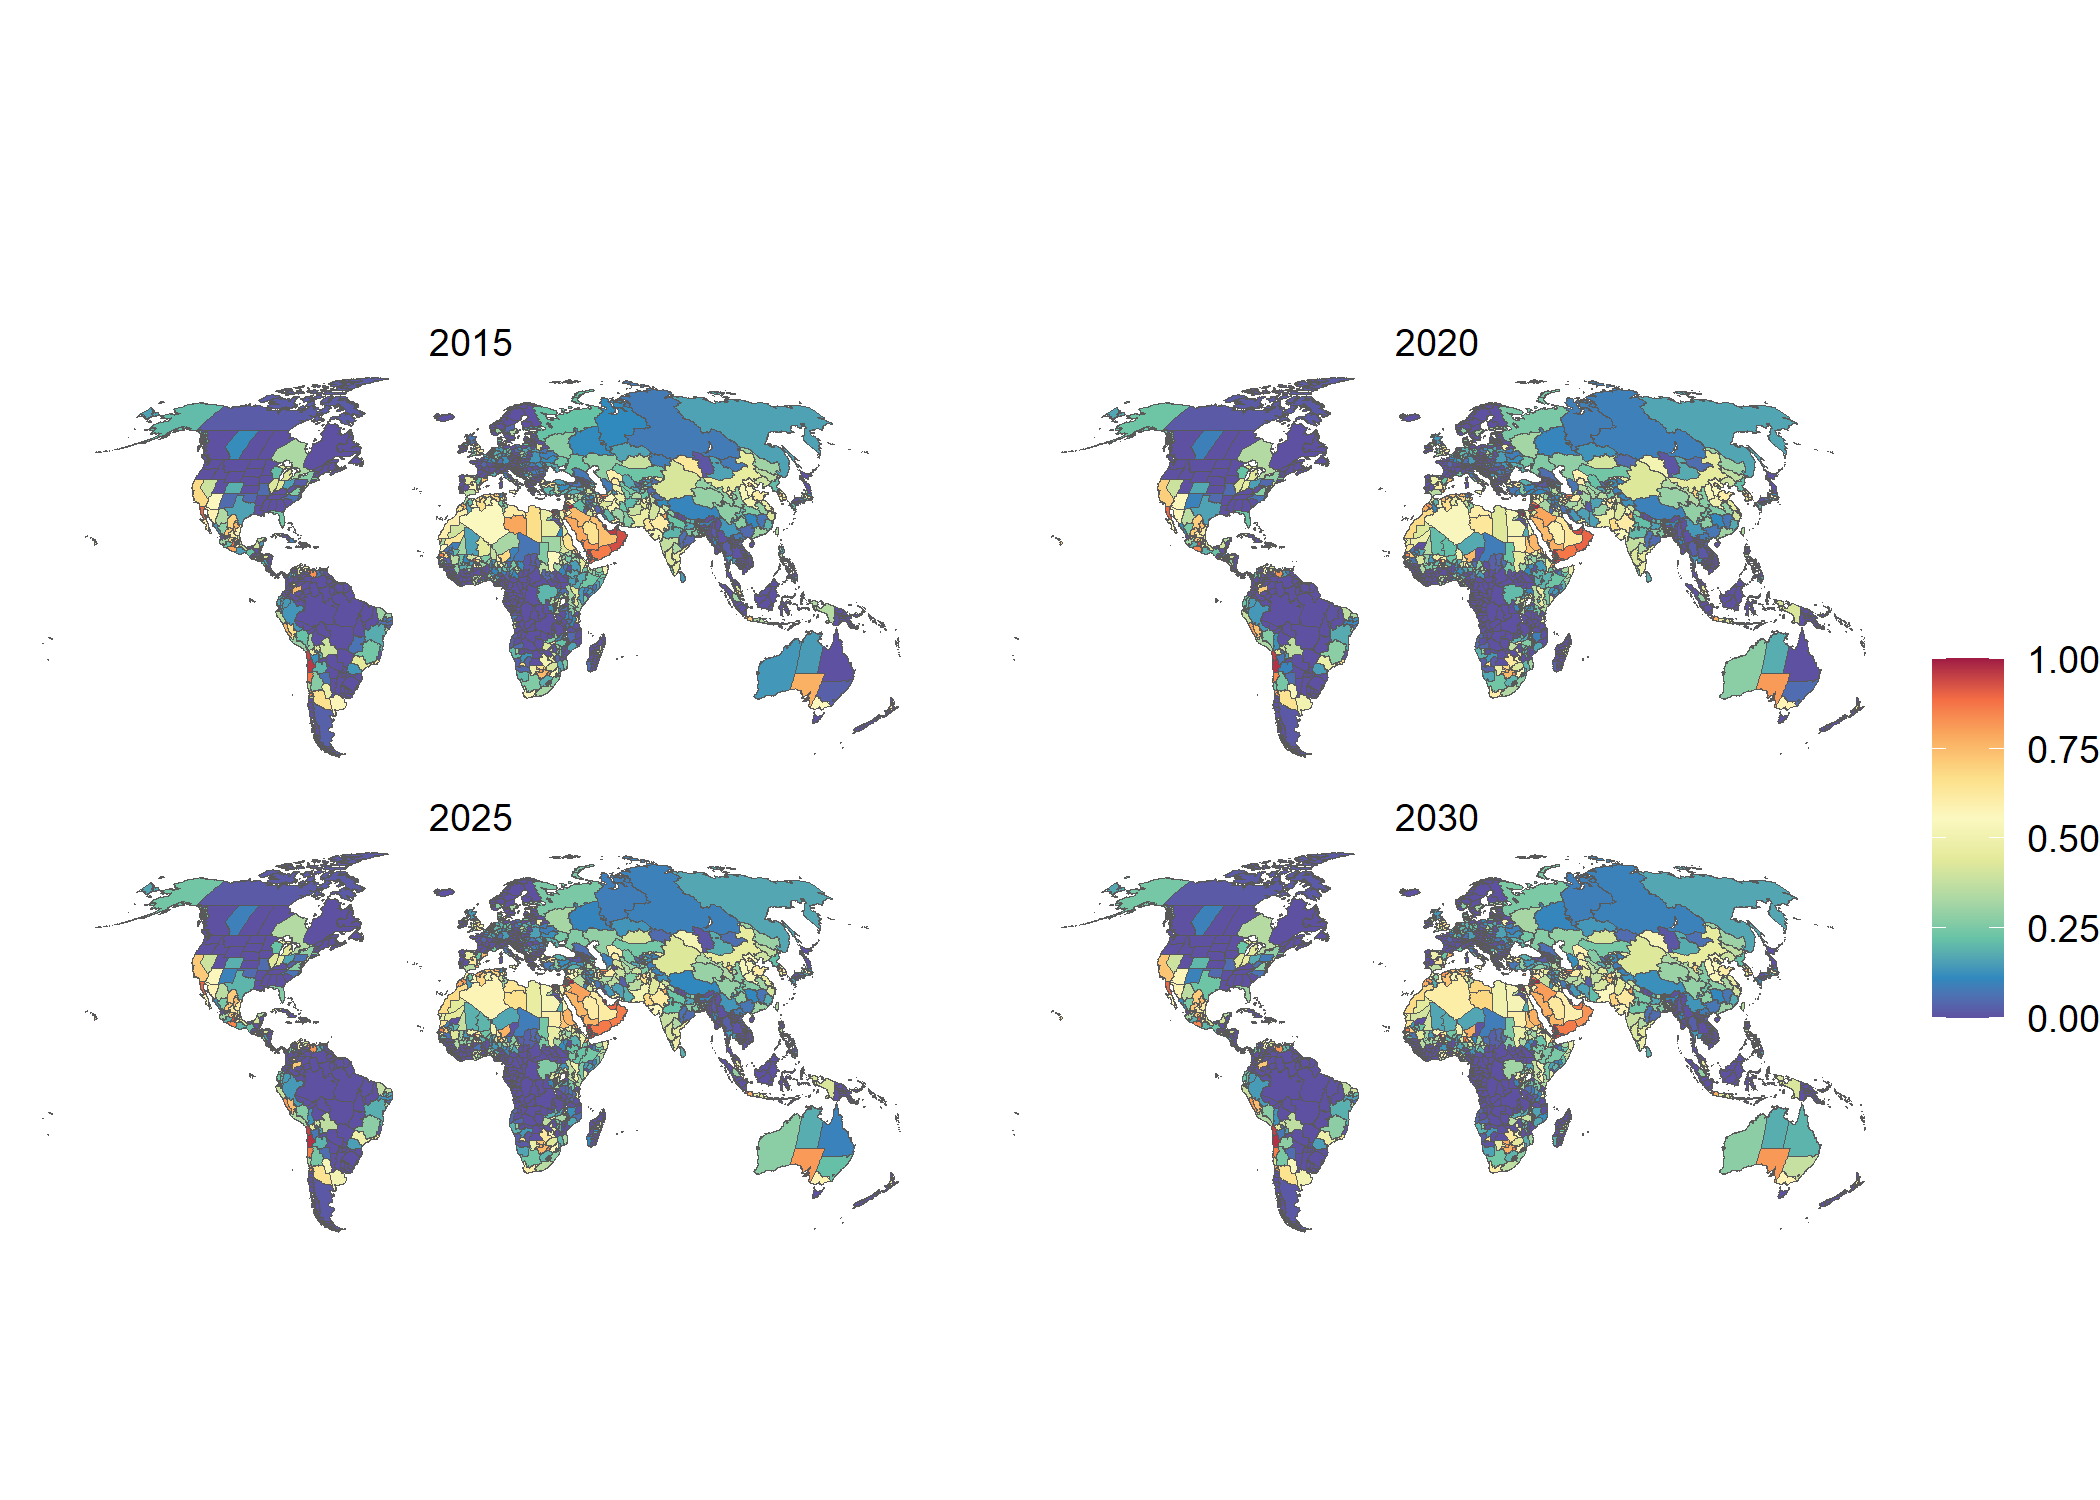
\includegraphics[width=\linewidth]{img/covars/ws_share.png}
  \caption{Water Scarcity Share}
\end{figure}


\pagebreak
\subsection{Mean Annual Precipitation and Mean Temperature}
For mean annual precipitation and temperature, we use data for the years 2010 to 2019 from the TerraClimate dataset \citep{abatzoglou2018terraclimate}, aggregated to each subnational area.  For data for the years 2020-2030, we use projections from models from the Inter-Sectoral Model Intercomparison Project \citep{warszawski2014inter}.  Specifically, we use the mean of an ensemble of bias-corrected projections under representative concentration pathway (RCP) 6.0.

\begin{figure}[H]
  \centering
  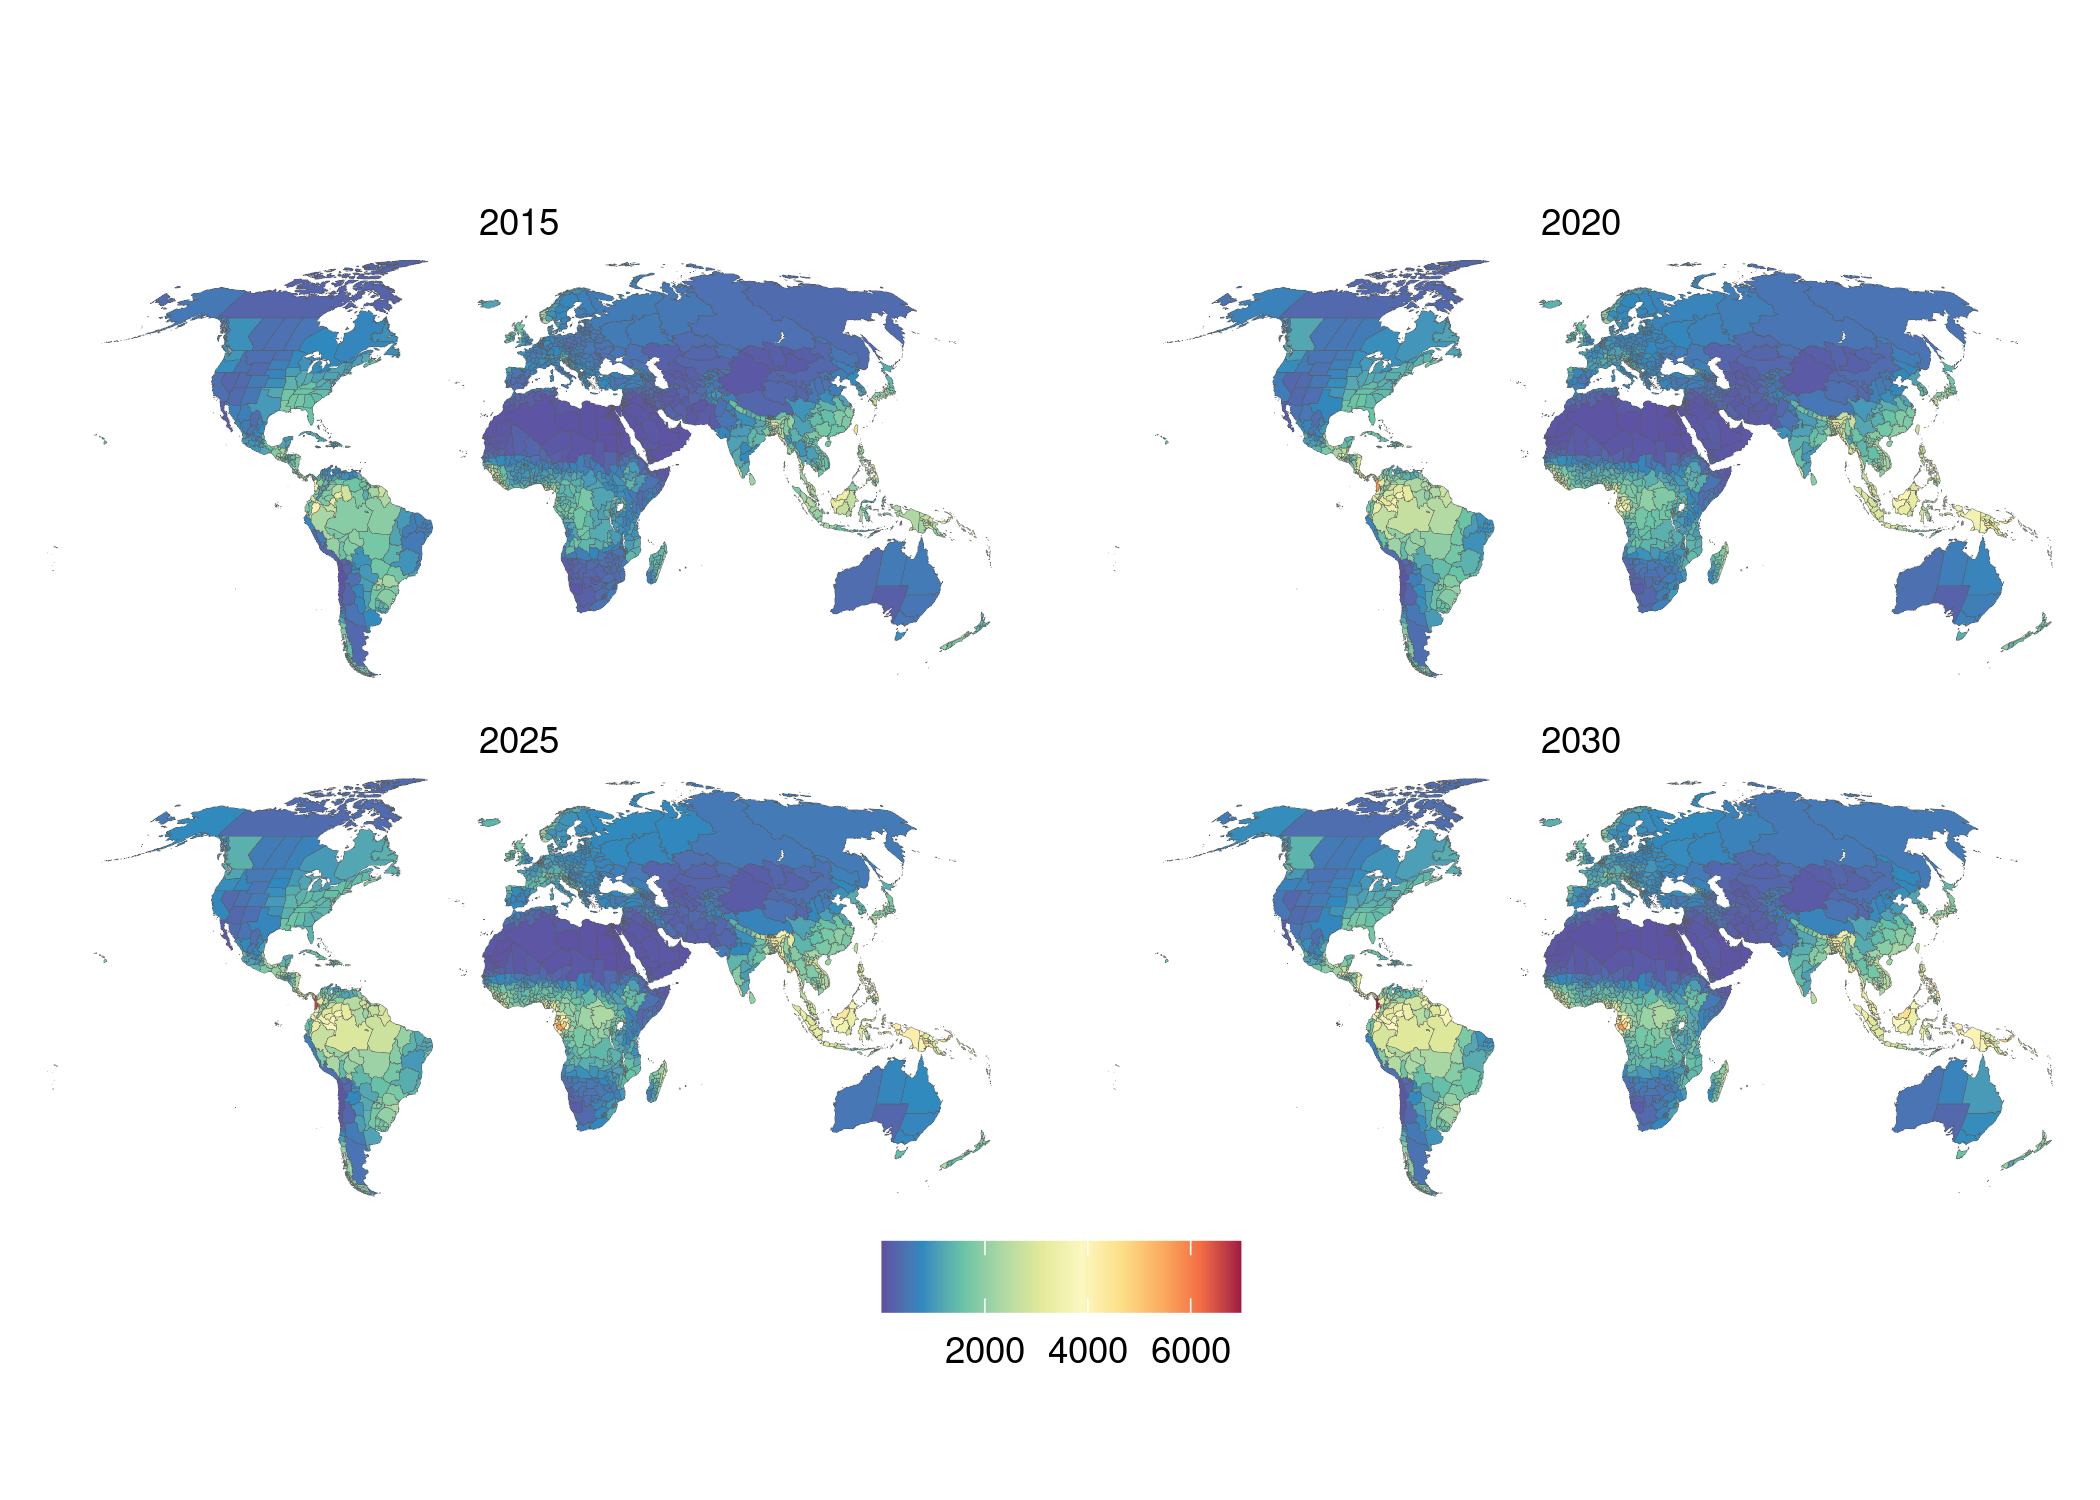
\includegraphics[width=\linewidth]{img/covars/precip.png}
  \caption{Mean Annual Precipitation}
\end{figure}

\begin{figure}[H]
  \centering
  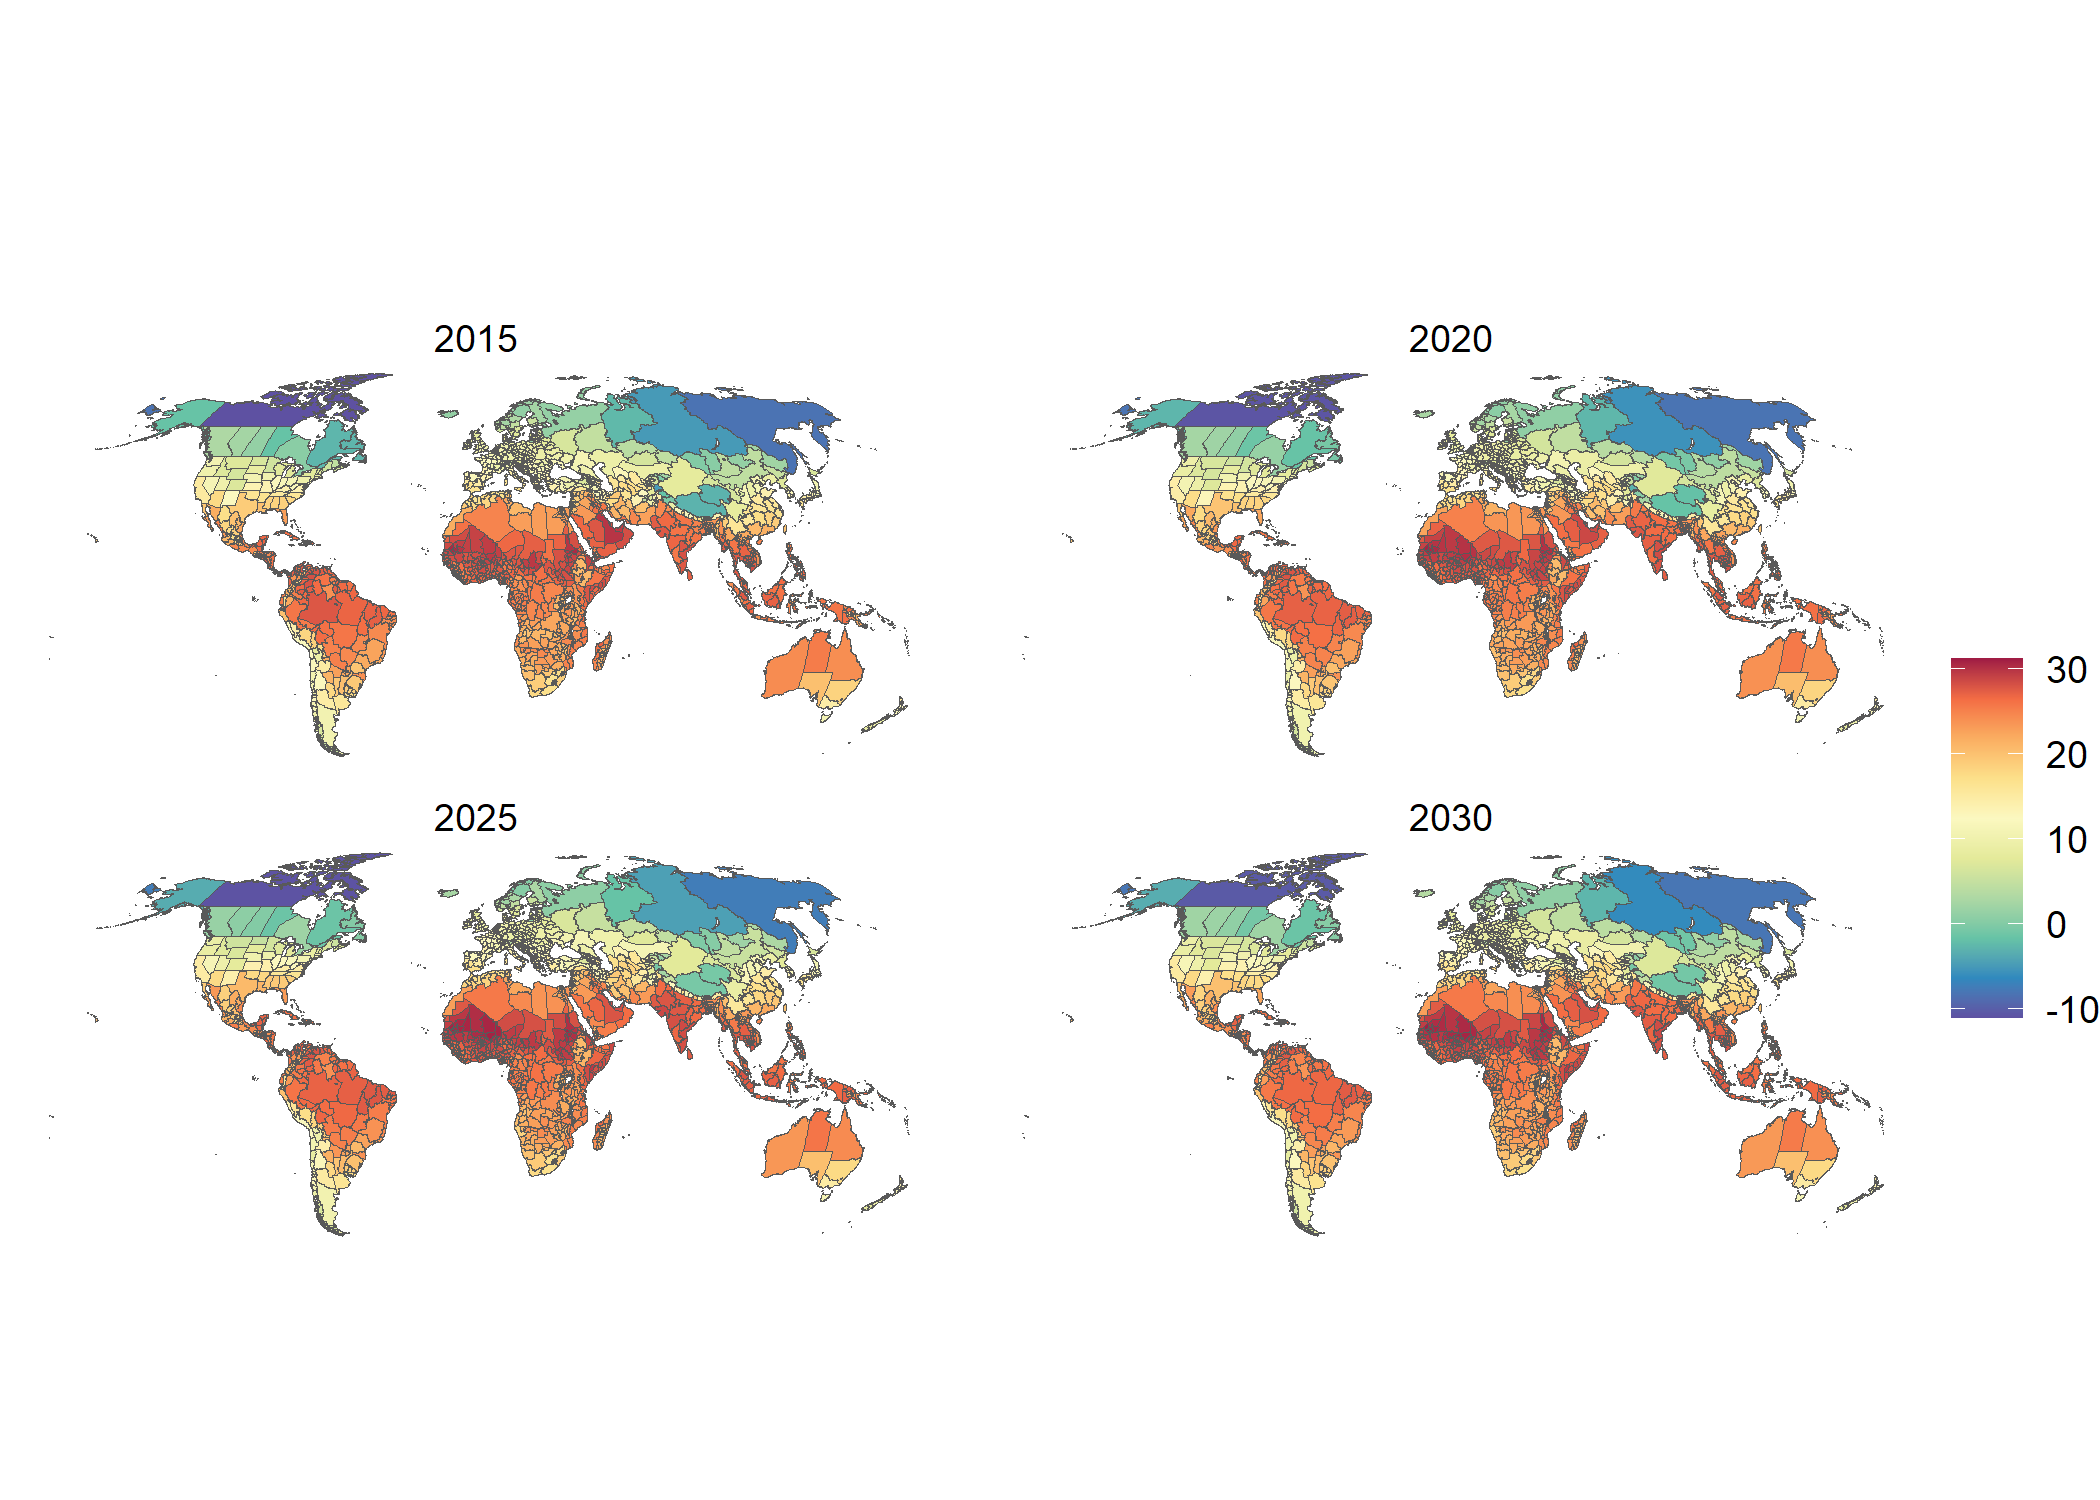
\includegraphics[width=\linewidth]{img/covars/tave.png}
  \caption{Mean Temperature (Celsius)}
\end{figure}

\pagebreak
\subsection{Topographic Ruggedness}
As a measure of accessibility, our models include the mean topographic ruggedness of each subnational area as a covariate. We obtain the variable using a gridded dataset of elevation from the USGS \citep{USGS1996} and calculate the index at each grid cell using the methodology from Riley et al. \citep{Riley1999}. We then aggregate the values for all the grid cells within each administrative area. The variable is constant in the estimation and projection period.

\begin{figure}[H]
  \centering
  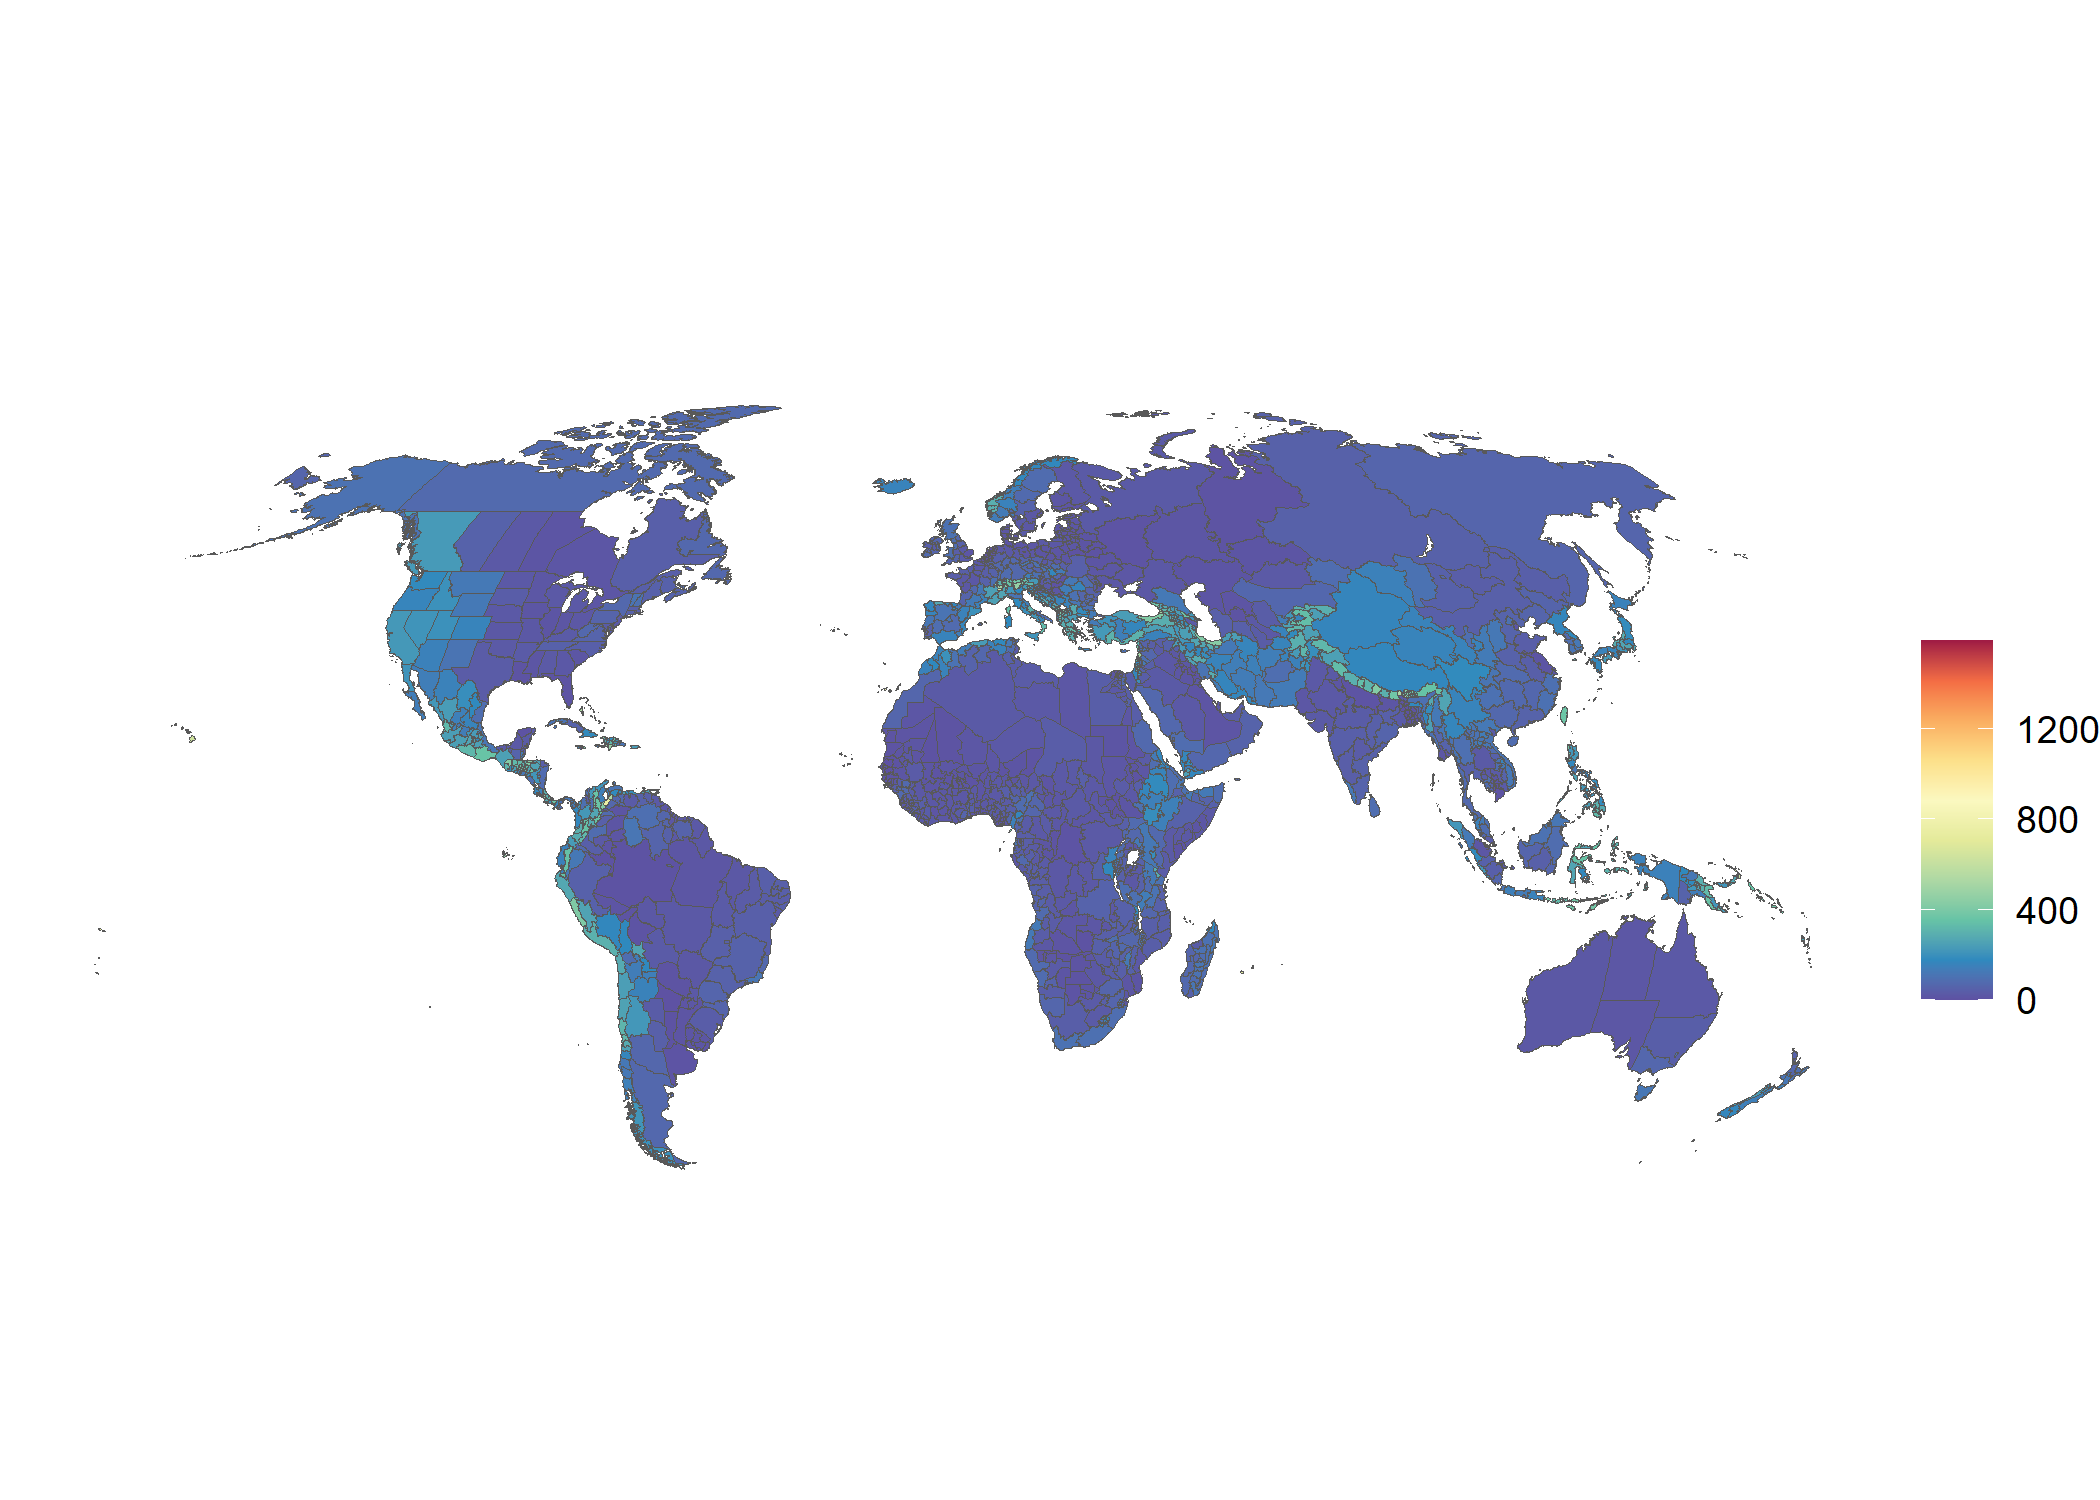
\includegraphics[width=\linewidth]{img/covars/ruggedness.png}
  \caption{Topographic ruggedness}
\end{figure}

\pagebreak
\subsection{Malaria (\textit{P. falciparum}) Mortality Rate}
We used data from Weiss et al. to estimate the mortality (deaths per 100,000 population per year) due to Malaria \citep{Weiss2019}, and aggregate the information at the level of subnational administrative area. Projections of malaria mortality are based on the AROC method.

\begin{figure}[H]
  \centering
  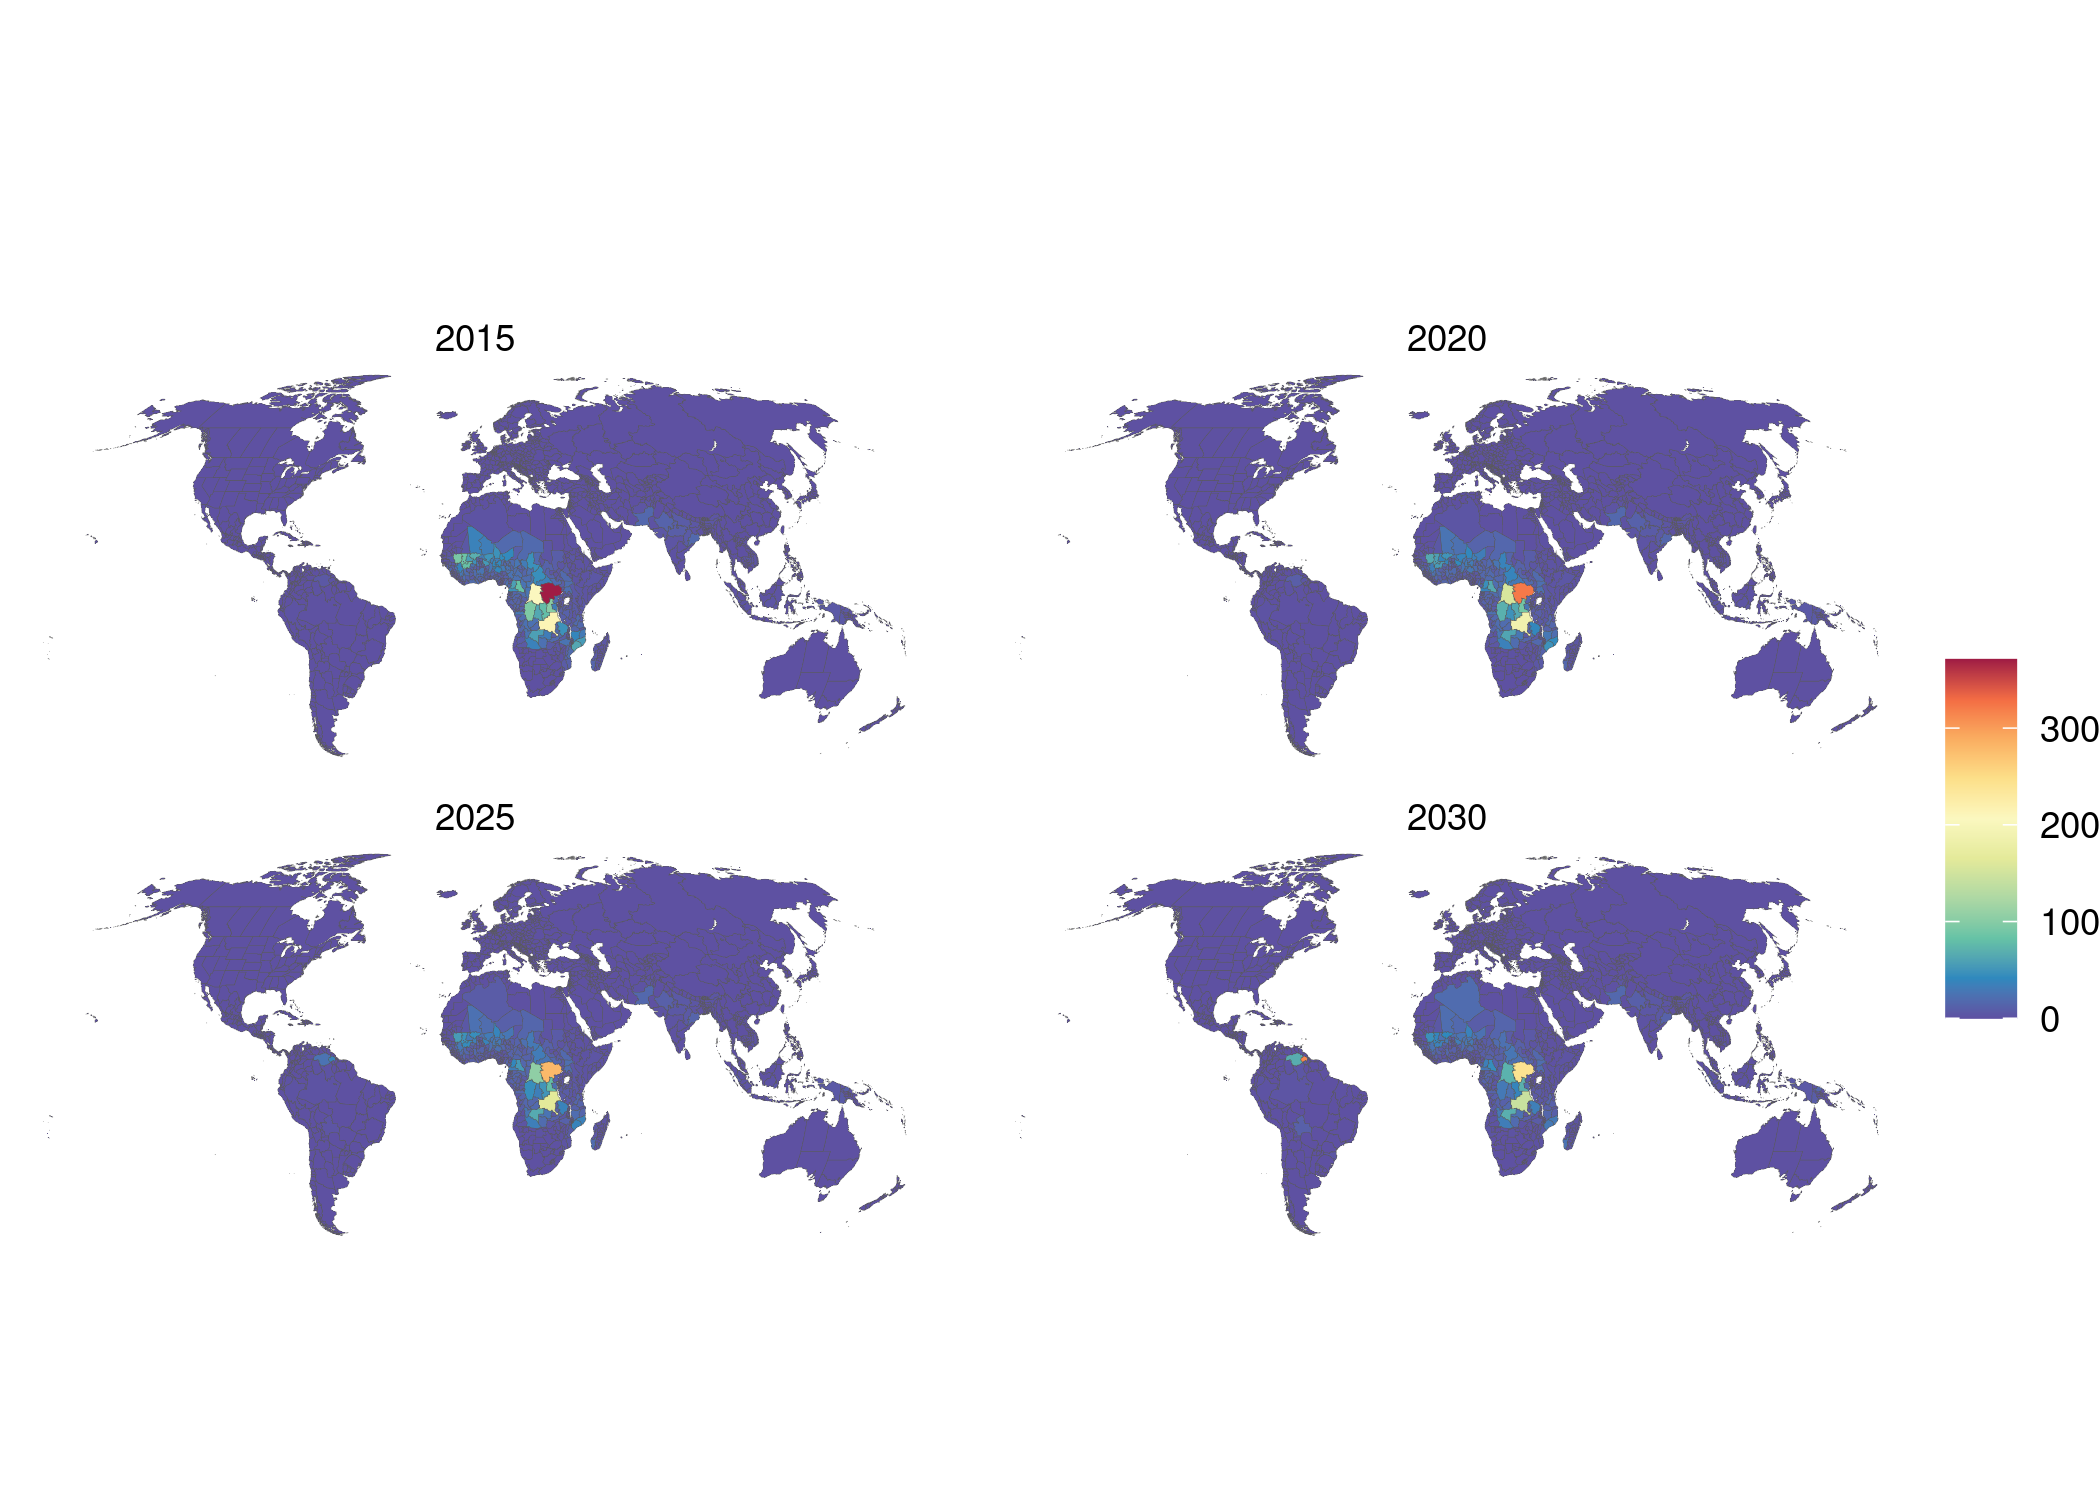
\includegraphics[width=\linewidth]{img/covars/mal_falciparum.png}
  \caption{Rate of mortality due to \textit{P. falciparum} Malaria}
\end{figure}

\pagebreak
\section{Description, Implementation and Validation of the Random Forest Regression Model}
The random forest regression is a machine learning method based on the creation of a large number of decision trees.  For each of the decision trees in a random forest model, observations are selected at random with replacement, a method known as bootstrap aggregating, or bagging, and features are also selected at random.  For the implementation we use the R-package \texttt{randomForestSRC} by Ishwaran and Kogalur \citep{ishwaran2019randomforestsrc}.

Because the outcome variables in our models, the rate of moderate or severe food insecurity, are a bounded outcome, we first used a logistic transformation to extend the range from $[0,1]$ to $(-\infty, \infty)$.  Then, after estimating the model, we used the inverse logit to convert the unbounded model predictions to a rate between 0 and 1.

To determine the best hyperparameters to model both moderate ands severe food insecurity, we use leave-one-out cross validation at the country level.  This involves running a separate model for each country, where we train a model on the remaining data from all of the other countries, and use that model to predict values for the country that was left out.  Then, across the predicted values for all countries, we evaluate the mean average error (MAE) and $R^2$ of the differences between observed rates of food insecurity and predictions from the cross validation models.

We evaluate models across a grid of hyperparameters, with combinations of: between 1 to 13 variables randomly selected as candidates for splitting a node (\texttt{mtry}), between 1 and 20 terminal node sizes (\texttt{nodesize}), and with a maximum tree depth (\texttt{depth}) between 1 to 13 nodes, as well as without any maximum tree depth.  For each model in cross validation, we used 1000 trees (\texttt{ntree}).  Due to the large size of the hyperparameter space, we sampled sets of hyperparameters randomly, eventually sampling about 50\% of all combinations of hyperparamters.  We found that the optimal model for moderate food insecurity had 16 average terminal nodes, 2 variables selected as candidates for splitting a node, and no maximum tree depth; the optimal model for severe food insecurity also had 2 variables selected as candidates for splitting a node and no maximum tree depth, but with only 14 average terminal.

After fitting models with cross validation, we evaluated the models performance and graphed a comparison between the observed and predicted values based on instances where individual countries were left out (See Fig. \ref{fig:rf_out-sample}), as well as for a model trained on the entire dataset, which can only be evaluated on in-sample data (See Fig. \ref{fig:rf_in-sample}).  Finally, Figure \ref{fig:mod-error} shows the model error converging and the number of trees increases.

\begin{figure}[H]
  \centering
  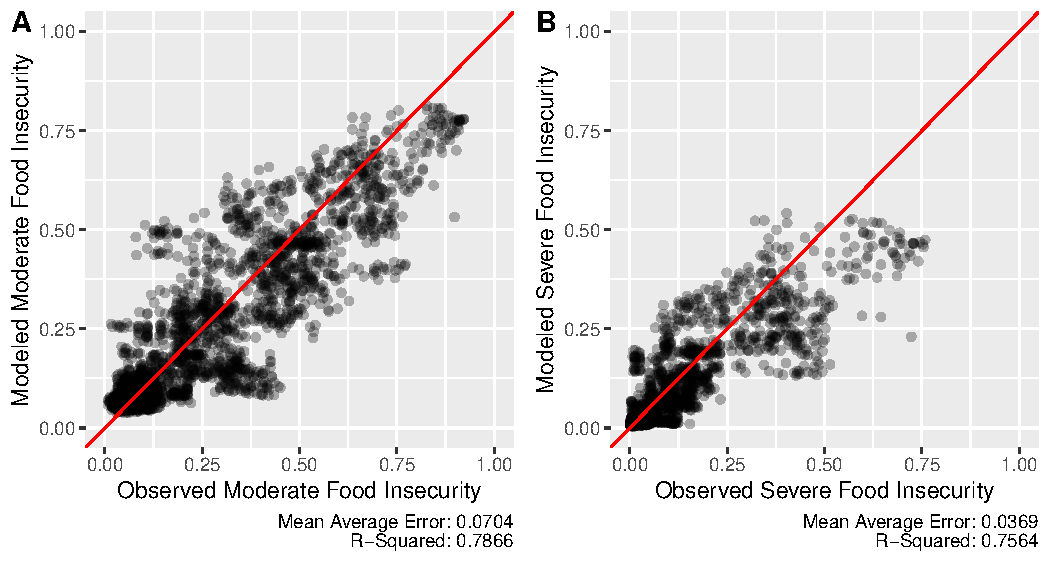
\includegraphics[width=\linewidth]{img/out-sample_rf.pdf}
  \caption{Out-of-sample fit of the random forest regression model, where predictions for each country are based on a model that did not include that country in the training data. Panel (A) shows the model for moderate food insecurity and panel (B) shows the model for severe food insecurity.}
  \label{fig:rf_out-sample}
\end{figure}

\begin{figure}[H]
  \centering
  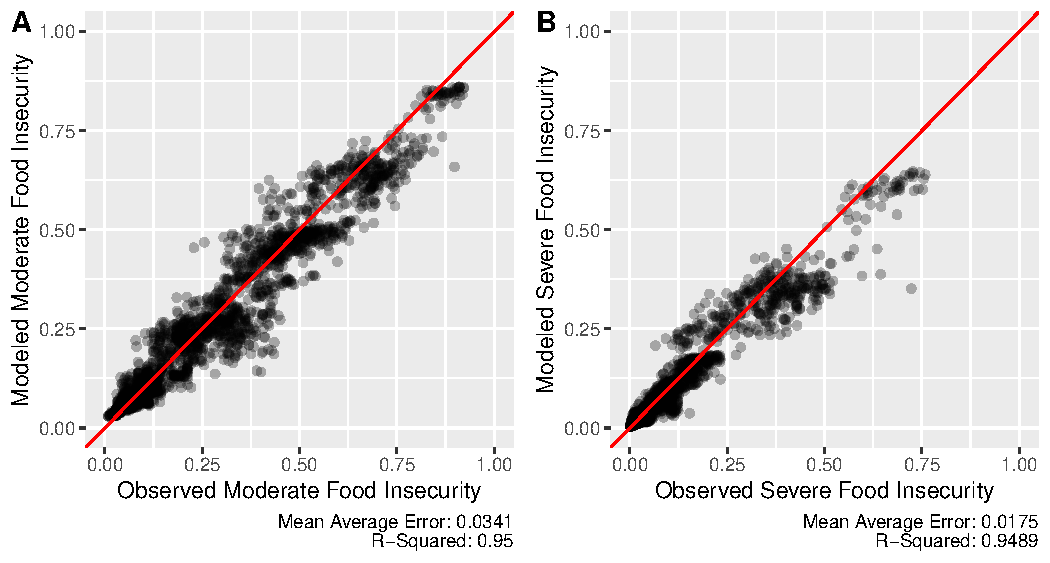
\includegraphics[width=\linewidth]{img/in-sample_rf.pdf}
  \caption{In-sample fit of the random forest regression model, where one model was trained on the entire dataset. Panel (A) shows the model for moderate food insecurity and panel (B) shows the model for severe food insecurity.}
  \label{fig:rf_in-sample}
\end{figure}

\begin{figure}[H]
  \centering
  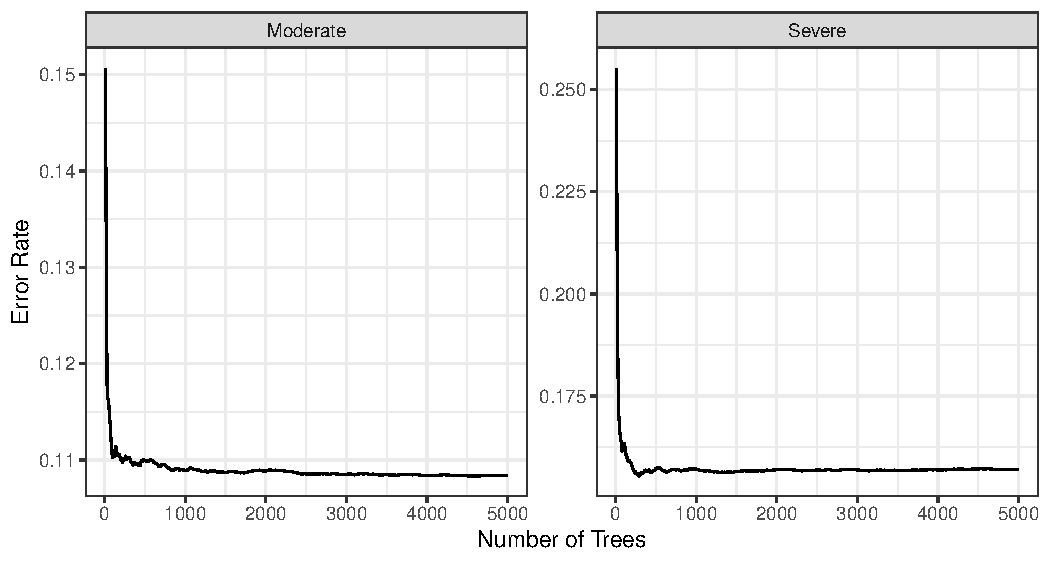
\includegraphics[width=\linewidth]{img/Error_Over_Training.pdf}
  \caption{Error rate of the random forest regression model as the number of trees in the model increases. Panel (A) shows the model for moderate food insecurity, and panel (B) shows the model for severe food insecurity.}
  \label{fig:mod-error}
\end{figure}

\end{document}

\printbibliography
